\begin{frontmatter}
	\chapter{O Método da Rigidez Direta (baseado em Deslocamentos)}
\end{frontmatter}

\section{O princípio do método}

Ao contrário do método das forças, em que se escrevem as equações de compatibilidade em função de ações incógnitas, o princípio que se adota no presente método é o de se exprimir diretamente o equilíbrio de cada nó do sistema estrutural em função de seus deslocamentos, \textit{agora considerados como incógnitas}. Estabelecendo-se assim, para um dado sistema estrutural, um modelo que se componha de \(ne\) elementos e \(nno\) nós, usados na definição dos elementos, gera-se então um sistema de equações com \(n\) incógnitas, onde \(n=nno \cdot ndofn\), sendo \(ndofn\) o número de graus de liberdade por nó do tipo de elemento estrutural.

Na Tabela \ref{ndofn} fornecem-se os valores de \textit{ndofn} para os diversos tipos de elementos reticulados segundo formulações clássicas de vigas.

\begin{table}[ht]
	\centering
	\caption{Valores de \textit{ndofn}}	\label{ndofn}
	\begin{tabular}{|l|l|}
		\hline
		treliça plana (em \(x_1x_2\))       & \(ndofn\!=\!2 \; (u_1, u_2)\)                                          \\ \hline
		treliça espacial (em \(x_1x_2x_3\)) & \(ndofn\!=\!3 \;(u_1, u_2, u_3)\)                                      \\ \hline
		viga (em \(x_1x_2\))                & \(ndofn\!=\!2 \; (u_2, \theta_3)\) ou \(=\!3 \; (u_1, u_2, \theta_3)\) \\ \hline
		pórtico plano (em \(x_1x_2\))       & \(ndofn=3 \; (u_1, u_2, \theta_3)\)                                    \\ \hline
		grelha (em \(x_1x_2\))              & \(ndofn\!=\!3 \;(\theta_1, \theta_2, u_3)\)                            \\ \hline
		pórtico espacial (em \(x_1x_2x_3\)) & \(ndofn=6 \; (u_1, u_2, u3, \theta_1, \theta_2, \theta_3)\)            \\ \hline
	\end{tabular}
\end{table}

\section{Rigidezes (conceito)}

Em geral, define-se a rigidez de elemento, \(k_{ij}\), como sendo a ação que surge na direção do \textit{i}-ésimo grau de liberdade do elemento em função de um deslocamento unitário (linear ou angular) segundo o seu \textit{j}-ésimo grau de liberdade. Por exemplo, para o elemento de pórtico plano mostrado na Fig. \ref{plfr1_gl}, no qual se indica a numeração de seus graus de liberdade, vê-se que para \(u_6=+1,0\) surgem as rigidezes mostradas na Fig. \ref{plfr1_rig} (ações de extremidade de elemento decorrentes do recalque angular).

\begin{figure}[!htbp]
	\begin{subfigure}[]{0.49\textwidth}
		\centering
		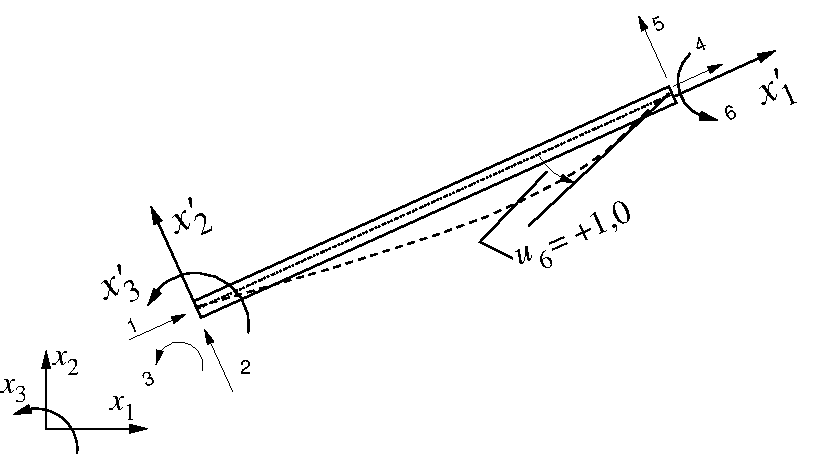
\includegraphics[scale=0.50]{img/elplanefr1_gl}
		\caption{\footnotesize Graus de liberdade} 		\label{plfr1_gl}
	\end{subfigure}
	\hfill
	\begin{subfigure}[]{0.49\textwidth}
		\centering
		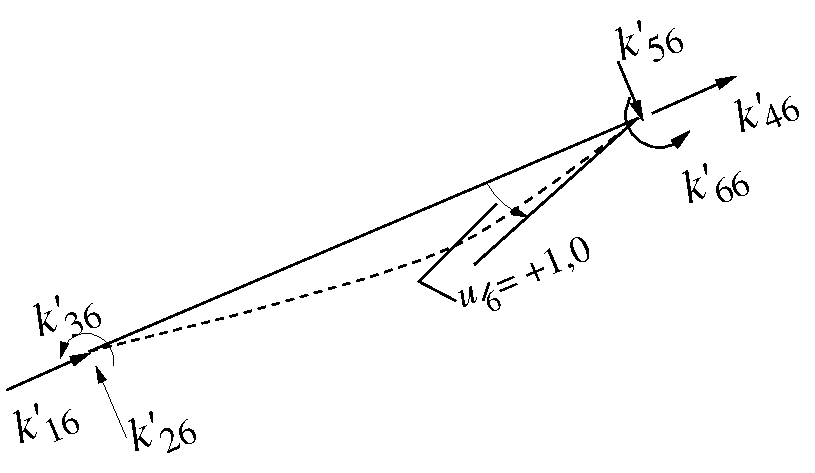
\includegraphics[scale=0.50]{img/elplanefr1_rig}
		\caption{\footnotesize Rigidezes}
		\label{plfr1_rig}
		\vspace{0cm}
	\end{subfigure}
	\caption{Elemento de pórtico plano} \label{plfr1}
\end{figure}

Essas rigidezes podem ser expressas tanto em relação ao referencial local (de elemento), \(x'_1x'_2x'_3\), como em relação ao referencial global (da estrutura), \(x_1x_2x_3\). No primeiro caso, obtém-se as rigidezes locais; no segundo, as globais. Naturalmente, os sinais (algébricos) das rigidezes são estabelecidos conforme a orientação dos eixos. Para o caso acima tem-se, por exemplo, que as rigidezes locais indicadas têm os seguintes sinais (algébricos): \(k'_{26}, k'_{36}\) e \(k'_{66}>0\) e \(k'_{56}<0\). Para o cálculo de seus valores, pode-se usar o método das forças. Tal procedimento será discutido detalhadamente em tópicos posteriores deste artigo.

De um modo geral, as rigidezes são calculadas em relação ao referencial local. Todavia, para o estabelecimento do sistema global faz-se necessário exprimi-las em relação ao referencial global (comum), pois os elementos do sistema estrutural podem possuir inclinações diferentes.

\section{Ações nodais externas}

Como mencionado inicialmente, a estratégia que se adota para o desenvolvimento da formulação de métodos dos deslocamentos fundamenta-se no estabelecimento de equações de equilíbrio para cada um dos nós do modelo. Desse modo, além dos esforços nodais internos, definidos pelas rigidezes, há naturalmente que se considerar também as ações nodais externas, decorrentes de cargas, variações de temperatura e deformações iniciais --- recalques são usualmente incluídos na análise como deslocamentos prescritos. Neste particular, 2 situações se distinguem, quais sejam: caso de cargas concentradas no nó e caso de ações atuantes no elemento (ao qual também se incluem variações de temperatura e deformações iniciais). No primeiro caso, por as cargas atuarem nos nós, poderão ser diretamente consideradas na equação de equilíbrio nodal. No segundo caso, cargas nodais equivalentes terão que ser determinadas. Tem-se, por exemplo, que para um elemento de pórtico plano submetido a uma carga genérica, \(q\) distribuída, surgem as ações nodais locais equivalentes indicadas na Fig. \ref{elloads}.

\begin{figure}[htbt!]
	\centering
	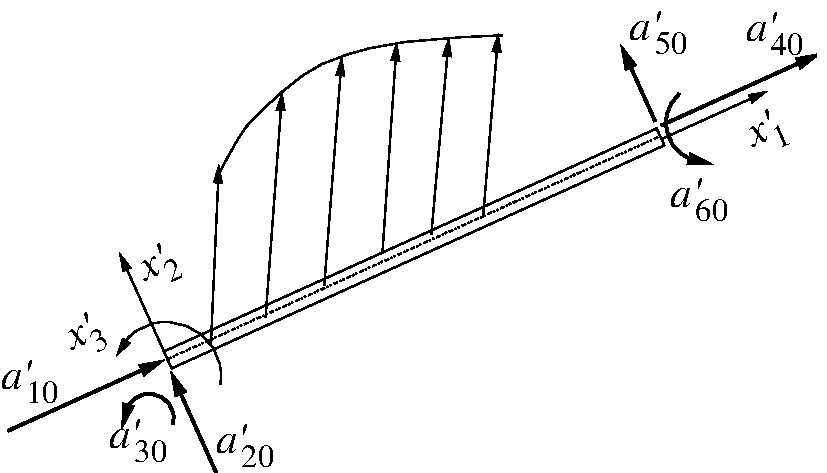
\includegraphics[scale=0.50]{img/planefrel1_loads}
	\caption{\footnotesize Cargas de elemento.}
	\label{elloads}
\end{figure}

Note-se que as ações nodais correspondem às reações de apoio da viga biengastada. Como no caso das rigidezes, seus valores podem também ser expressados via transformação de rotação em relação ao sistema global, e para a obtenção desses valores, igualmente usa-se o método das forças.

\section{Transformação de rotação de eixos}

Seja \(\mathbf{v}\) um vetor expresso em relação a um referencial \(S\) e  \(\mathbf{v}'\) esse mesmo vetor expresso em relação a um referencial \(S'\). Para o caso em que os \(n\) eixos de cada um desses sistemas de referência são mutuamente ortogonais entre si, verifica-se que:

\[
	\begin{aligned}
		\mathbf{v}' & =\mathbf{R} \cdot \mathbf{v}    \\
		\mathbf{v}      & =\mathbf{R}^T \cdot \mathbf{v'}
	\end{aligned}
	\;,
\]
\noindent  onde

\medskip

\[
	\mathbf{R}=
	\left [\;\;
		\begin{matrix}
			\lambda_{11} & \lambda_{12} & \cdots & \lambda_{1n} \\
			\lambda_{21} & \lambda_{22} & \cdots & \lambda_{2n} \\
			\vdots       & \vdots       & \ddots & \vdots       \\
			\lambda_{n1} & \lambda_{n2} & \cdots & \lambda_{nn} \\
		\end{matrix}
		\right ] \; , \quad
	\lambda_{ij}=\cos(x'_i,x_j)\; .
\]

\noindent em que \(\mathbf{R}\) é a matriz (ou transformação) de rotação de eixos. Para a formulação em questão, de fato, apenas os casos de \(n=2\) (bidimensional) e \(n=3\) (tridimensional) ocorrerão.
Para o caso \(2D\) tem-se:

\begin{minipage}{0.5\textwidth}
	\[
		\mathbf{R}
		=
		\left [\;\;
			\begin{matrix}
				\cos \theta                & \cos(\frac{\pi}{2}-\theta) \\
				\cos(\frac{\pi}{2}+\theta) & \cos \theta                \\
			\end{matrix}
			\right ]
		=
		\left [ \;\;
			\begin{matrix}
				\cos \theta  & \sin \theta \\
				-\sin \theta & \cos \theta \\
			\end{matrix}
			\right ]
	\]
\end{minipage}
\hspace{0.5cm}
\begin{minipage}{0.4\textwidth}
	\begin{center}
		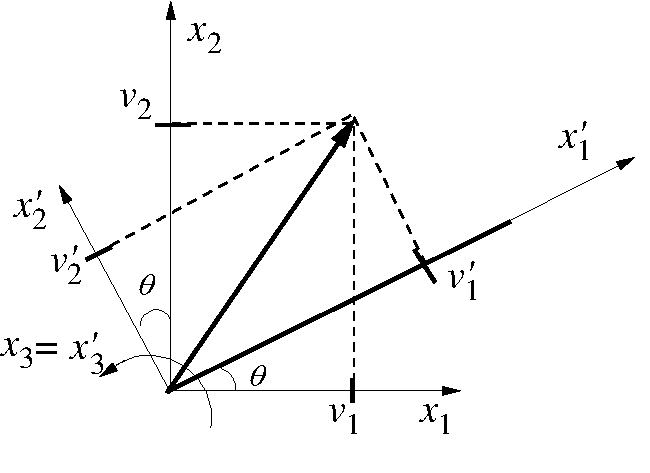
\includegraphics[scale=0.50]{img/rot2D}
		\captionof{figure}{Rotação de eixos (\(n\!=\!2\)).}
		\label{rot_eixos}
		\vspace{12pt}
	\end{center}
\end{minipage}

\bigskip

Para \(n=3\) (ou mesmo \(n>3\)), a determinação da matriz de rotação também não oferece qualquer dificuldade. Na verdade, dados os vetores unitários \(\bf{e}_i\) e \(\bf{e'}_i\) definindo os referenciais S e S', tem-se:

\[
	\lambda_{ij}
	=
	\cos(\mathbf{e'}_i,\mathbf{e}_j)=(\mathbf{e'}_i,\mathbf{e}_j) \quad \textrm{(produto escalar entre  \(\mathbf{e}'_i\) e \(\mathbf{e}_j\)) .}
\]
Ressalta-se ainda que como S e S' são mutuamente ortogonais, então \textbf{R} é uma matriz ortogonal. Assim,
\(\mathbf{R}^{-1}\!=\!\mathbf{R}^{T}\). No caso de rotação de matrizes de S para S' e de S' para S, usam-se as relações:

\[
	{\mathbf{A'}}=\mathbf{R}\mathbf{A}\mathbf{R}^{T} , \quad
	\mathbf{A}=\mathbf{R}^{T}{\mathbf{A'}}\mathbf{R}
\]

\medskip

Note-se que para \(\mathbf{v}_2=\mathbf{A}\mathbf{v}_1\), obtém-se:

\[
	\mathbf{R}\mathbf{v}_2=(\mathbf{R}\mathbf{A}\mathbf{R}^{T})(\mathbf{R}\mathbf{v}_1)
	\Rightarrow
	\mathbf{v'}_2=\mathbf{A'}\mathbf{v'}_1
	\; .
\]

A matriz \(\mathbf{A}'\), referenciada a \(S'\), é portanto a transformação matemática que associa \(\mathbf{v}'_1\) a \(\mathbf{v}'_2\), os quais no referencial \(S\), dados por \(\mathbf{v}_1\) a \(\mathbf{v}_2\) respectivamente, estavam associados pela transformação \(\mathbf{A}\), referenciada a \(S\).

Abaixo indicam-se as matrizes de rotação necessárias ao desenvolvimento da formulação dos diversos tipos de elementos reticulados. Tem-se:

\begin{minipage}{0.3\textwidth}
	a) Treliça plana (\textit{ndofn}=2)

	\[ \mathbf{R}=\left [\;\; \begin{matrix}
				\cos \theta  & \sin \theta \\
				-\sin \theta & \cos \theta \\
			\end{matrix}\right ] \]
\end{minipage}  \hspace{0.5cm}
\begin{minipage}{0.6\textwidth}
	\begin{center}
		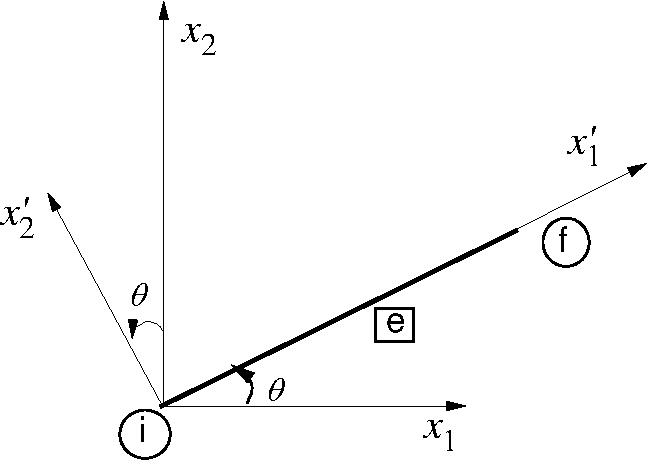
\includegraphics[scale=0.45]{img/rot-trel2D}
		\captionof{figure}{Sistemas de referência local e global}
		\label{rot_eixos_tr2d}   \vspace{12pt}
	\end{center}
\end{minipage}

\begin{minipage}{0.49\textwidth}
	b) Viga, pórtico plano e grelha (\textit{ndofn}=3, \(x'_3\equiv x3\))

	\[
		\mathbf{R}
		=
		\left [\;\;
			\begin{matrix}
				\cos \theta  & \sin \theta & 0 \\
				-\sin \theta & \cos \theta & 0 \\
				0            & 0           & 1 \\
			\end{matrix}
			\right ]
	\]
\end{minipage}  \hspace{-0.5cm}%%% to prevent a space
\begin{minipage}{0.49\textwidth}
	\begin{center} %\hspace{-1,0cm}
		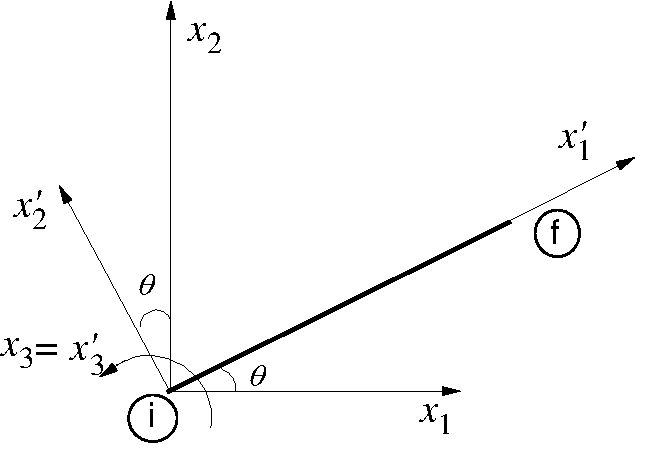
\includegraphics[scale=0.45]{img/rot-port2D}
		\captionof{figure}{Sistemas de referência local e global}
		\label{rot_eixos_fr2d}   \vspace{12pt}
	\end{center}
\end{minipage}

\

\begin{minipage}{0.49\textwidth}
	c) Pórticos e treliças espaciais

	\[\bf{R}=\left [\;\; \begin{matrix}
				\lambda_{11} & \lambda_{12} & \lambda_{13} \\
				\lambda_{21} & \lambda_{22} & \lambda_{23} \\
				\lambda_{31} & \lambda_{32} & \lambda_{33} \\
			\end{matrix}\right ]\; , \quad \textrm{com \(\lambda_{ij}\!=\!(\mathbf{e}'_i,\mathbf{e}_j)\) }  \]
\end{minipage}  \hspace{-0.5cm}%%% to prevent a space
\begin{minipage}{0.49\textwidth}
	\begin{center} %\hspace{-1,0cm}
		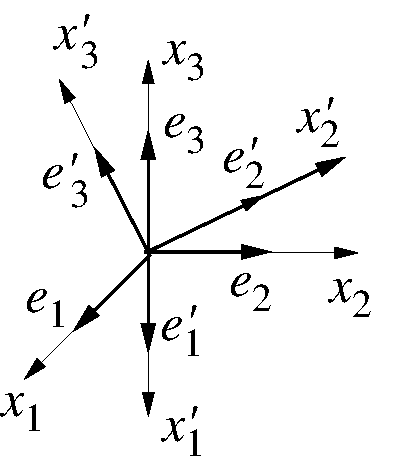
\includegraphics[scale=0.45]{img/rot-port3D}
		\captionof{figure}{Sistemas de referência local e global}
		\label{rot_eixos3d}   \vspace{12pt}
	\end{center}
\end{minipage}

\

Para pórticos espaciais adotam-se, em geral, os seguintes eixos locais: \
\(x'_1=\) eixo centroidal do elemento;
\(x'_2\) e \(x'_3\) são eixos principais de inércia das seções dos elementos. Ressalta-se, porém, que eixos não-principais e não centroidais são, na verdade, necessários em situações práticas de análise de pórticos espaciais, onde e.g. a linha neutra da seção pode variar continuamente em razão de não-linearidades físicas. Para pórticos planos e grelhas, o eixo local \(x'_2\), de todas as seções da estrutura, será necessariamente principal; já  \(x'_1\) poderá ser o eixo centroidal ou não, sendo eixos não-centroidais mais relevantes em aplicações práticas, como explicado acima.

\

\noindent \textbf{Exercício}.
Mostre como se obtêm as matrizes de rotação dadas acima para os elementos de treliças e de pórticos planos e espaciais.

\section{Matriz de Rigidez de Elemento}

Define-se a matriz de rigidez do elemento, \(\mathbf{K}^{(e)}\), como sendo a transformação que associa os deslocamentos de extremidade de elemento às respectivas ações (esforços internos). Considerando-se a definição de coeficientes de rigidez, \(k_{ij}\), pode-se escrever (em notação indicial) para o referencial local:

\begin{minipage}{0.44\textwidth}
	\[ a'_i=\sum_{j=1}^{2\cdot ndofn}k'_{ij}u'_j, \textrm{com \(i\!=\!1,\cdots,ndofn\)} \;. \]
	\

	\noindent Ou em notação vetorial (particionada conforme os grupos de variáveis dos nós inicial, \(i\), e final, \(f\)):
	\[\left [ \;\;\begin{matrix}
				\mathbf{a}'_i \\
				\mathbf{a}'_f \\
			\end{matrix}\right ]
		= \left [\;\; \begin{matrix}
				{\mathbf{K'}}_{ii}^{(e)}                     & {\mathbf{K'}}_{if}^{(e)} \\
				{\mathbf{K'}}_{fi}^{(e)} & {\mathbf{K'}}_{ff}^{(e)} \\
			\end{matrix}\right ]
		\cdot \left [\;\; \begin{matrix}
				\mathbf{u}'_i \\
				\mathbf{u}'_f \\
			\end{matrix}\right ] \; , \]
\end{minipage}  \hspace{-0.5cm}
\begin{minipage}{0.55\textwidth}
	\begin{center}
		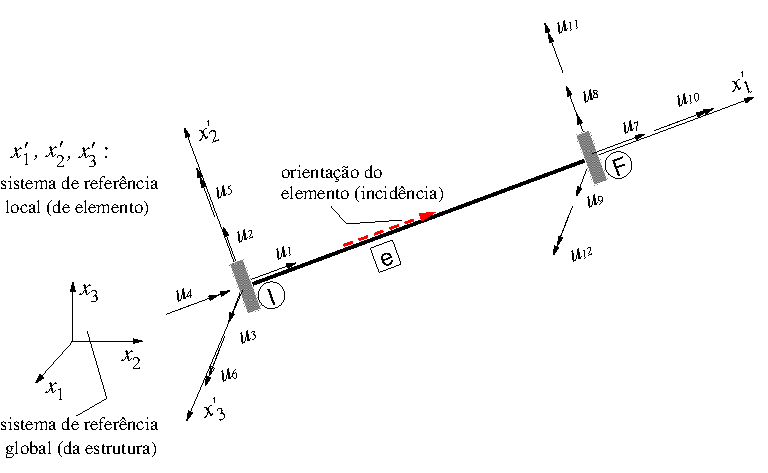
\includegraphics[scale=0.6]{img/fr3Del1}
		\captionof{figure}{ Elemento de pórtico espacial}
		\label{el3d}   \vspace{12pt}
	\end{center}
\end{minipage}
\clearpage
\noindent Em forma não particionada tem-se:

\

\[ {\mathbf{a'}}=\mathbf{K}'^{(e)}{\mathbf{u'}} \; ,\]

\noindent onde \(\mathbf{a}'\) é o vetor de ações locais de extremidade de elemento (esforços internos), \(\mathbf{K}'^{(e)}\) é a matriz de rigidez local do elemento e \(\mathbf{u}'\) é o vetor de deslocamentos locais de elemento.

\

\noindent Observações:
\begin{enumerate}
	\item {Note-se que \(\mathbf{a}'_i, \mathbf{a}'_f, \mathbf{u}'_i\) e \(\mathbf{u}'_f\) são vetores com \textit{ndofn} componentes. Assim, a matriz de rigidez é da ordem \(n=nnoel\cdot ndofn\), onde, no caso, \(nnoel=2\) (número de nós por elemento).}

	\item  Para cada tipo de elemento estrutural, uma numeração própria de seus graus de liberdade pode ser estabelecida. Aqui, adotar-se-ão as seguintes numerações dos graus de liberdade:

	      \

	      \begin{figure}[htb!]
		      \begin{subfigure}{0.30\textwidth}
			      \begin{center} %\hspace{-1,0cm}
				      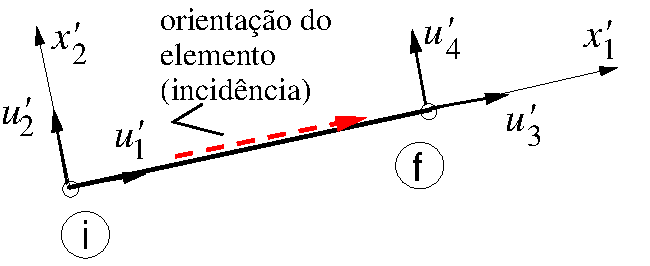
\includegraphics[scale=0.4]{img/numeltrl2d}
				      \caption{\footnotesize Treliças planas}
				      \label{numeltrl2d}   \vspace{12pt}
			      \end{center}
		      \end{subfigure}  \hspace{0cm}%%% to prevent a space
		      \begin{subfigure}{0.35\textwidth}
			      \begin{center} %\hspace{-1,0cm}
				      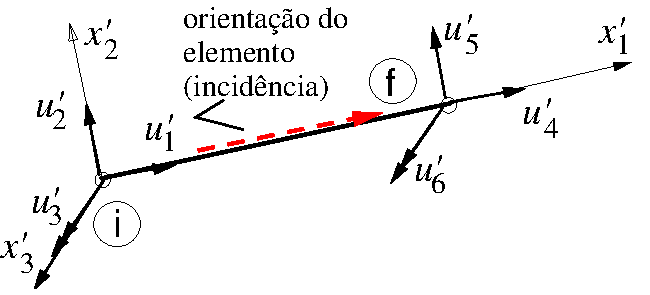
\includegraphics[scale=0.40]{img/numelfr2d}
				      \caption{\footnotesize Vigas e Pórticos planos}
				      \label{numelfr2d}   \vspace{12pt}
			      \end{center}
		      \end{subfigure}
		      \begin{subfigure}{0.30\textwidth}
			      \begin{center} %\hspace{-1,0cm}
				      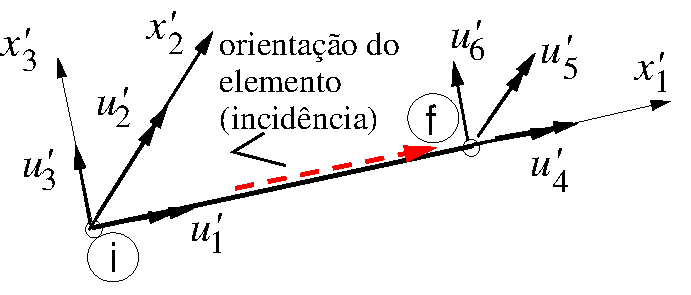
\includegraphics[scale=0.4]{img/numelgrelha}
				      \caption{\footnotesize Grelhas}
				      \label{numelgr}   \vspace{12pt}
			      \end{center}
		      \end{subfigure}
		      \caption{Numeração dos graus de liberdade de elementos reticulados}
		      \label{numgl}
	      \end{figure}

	      A numeração de pórtico espacial é aquela indicada na Fig. \ref{el3d}. Note-se que, para treliças (planas ou espaciais) os eixos locais (de elemento) não precisam ser principais (podem ser quaisquer). Para todos os outros tipos de elemento (vigas, pórticos planos e espaciais, e grelhas), eixos locais não-centroidais e não-principais demandam formulações generalizadas de flexão para o correto estabelecimento das matrizes de rigidez.

	\item Na verdade, as matrizes de rigidez de elemento são inicialmente obtidas para o referencial local S'. Via transformação de rotação elas podem, contudo, ser facilmente expressas em relação ao referencial global S. Tem-se:

	      \medskip

	      \[
		      \left\{\;\; \begin{matrix}
			      {\mathbf{a'}}_i={\mathbf{K'}}_{ii}^{(e)}{\mathbf{u'}}_i + {\mathbf{K'}}_{if}^{(e)}{\mathbf{u'}}_f          \\
			      {\mathbf{a'}}_f={\mathbf{K'}}_{fi}^{(e)}{\mathbf{u'}}_i + {\mathbf{K'}}_{ff}^{(e)}{\mathbf{u'}}_f \\
		      \end{matrix}\right.
		      \;,
	      \]

	      \medskip

	      \[
		      \left\{\;\; \begin{matrix}
			      \mathbf{R}^{T}{\mathbf{a'}}_i=(\mathbf{R}^{T}{\mathbf{K'}}_{ii}^{(e)}\mathbf{R})(\mathbf{R}^{T}{\mathbf{u'}}_i) + (\mathbf{R}^{T}{\mathbf{K'}}_{if}^{(e)}\mathbf{R})(\mathbf{R}^{T}{\mathbf{u'}}_f) \\
			      \mathbf{R}^{T}{\mathbf{a'}}_f=(\mathbf{R}^{T}{\mathbf{K'}}_{fi}^{(e)}\mathbf{R})(\mathbf{R}^{T}{\mathbf{u'}}_i) + (\mathbf{R}^{T}{\mathbf{K'}}_{ff}^{(e)}\mathbf{R})(\mathbf{R}^{T}{\mathbf{u'}}_f) \\
		      \end{matrix}\right.
		      \;,
	      \]

	      \medskip

	      \[
		      \begin{bmatrix}
			      \mathbf{a}_i \\
			      \mathbf{a}_f \\
		      \end{bmatrix}
		      =
		      \begin{bmatrix}
			      \mathbf{R}^{T}{\mathbf{K'}}_{ii}^{(e)}\mathbf{R} & \mathbf{R}^{T}{\mathbf{K'}}_{if}^{(e)}\mathbf{R} \\
			      \mathbf{R}^{T}\bf{K'}_{fi}^{(e)}\mathbf{R}   & \mathbf{R}^{T}{\mathbf{K'}}_{ff}^{(e)}\mathbf{R} \\
		      \end{bmatrix}
		      \begin{bmatrix}
			      \mathbf{u}_i \\
			      \mathbf{u}_f \\
		      \end{bmatrix}
		      =
		      \begin{bmatrix}
			      \mathbf{K}_{ii}^{(e)} & \mathbf{K}_{if}^{(e)} \\
			      \mathbf{K}_{fi}^{(e)} & \mathbf{K}_{ff}^{(e)} \\
		      \end{bmatrix}
		      \begin{bmatrix}
			      \mathbf{u}_i \\
			      \mathbf{u}_f \\
		      \end{bmatrix}
		      \;,
	      \]

	      \medskip

	      \[ \mathbf{a}=\mathbf{K}^{(e)}\mathbf{u} \;, \]

	      onde \(\mathbf{a}\) é o vetor de ações globais de extremidade de elemento; \(\mathbf{K}^{(e)}\) é a matriz de rigidez global do elemento e \(\mathbf{u}\) é o vetor de deslocamentos globais de elemento.

	\item Do teorema de reciprocidade para rigidezes, verifica-se que

	      \[ k'_{ij}=k'_{ji} \; . \]

	      Assim, \({\mathbf{K'}}_{fi}^{(e)}={\mathbf{K'}}_{if}^{(e),T}\), e também

	      \[ \mathbf{K}_{if}^{(e),T}=(\mathbf{R}^{T}{\mathbf{K'}}_{if}^{(e)}\mathbf{R})^T=\mathbf{R}^{T}{\mathbf{K'}}_{if}^{(e),T}\mathbf{R}=\mathbf{R}^{T}{\mathbf{K'}}_{fi}^{(e)}\mathbf{R}=\mathbf{K}_{fi}^{(e)} \; .\]

	      Portanto, a matriz de rigidez de elemento é simétrica.

	\item Nota-se que se o elemento, após atuação de deslocamentos, permanecer indeformado, ou seja, se estiver sob campo de deslocamento de corpo rígido, então, obviamente, as suas ações de extremidade, \(\mathbf{a}_i\) e \(\mathbf{a}_f\) (ou \({\mathbf{a'}}_i\) e \({\mathbf{a'}}_f\)), em função de seus deslocamentos de extremidade (deformação do elemento), serão nulas. Tem-se, portanto:

	      \begin{minipage}{0.35\textwidth}
		      \[\left\{ \; \begin{aligned}
				      \mathbf{a} & =\mathbf{K}^{(e)}\mathbf{u}^{(e)}=\mathbf{0} \; ,       \\
				      \mathbf{a} & ={\mathbf{K'}}^{(e)}{\mathbf{u'}}^{(e)}=\mathbf{0} \; .\end{aligned}
			      \right. \]

		      \medskip

		      Logo, \(|\mathbf{K}^{(e)}|=|\mathbf{K'}^{(e)}|=0\). A matriz de rigidez de elemento é singular.
	      \end{minipage}
	      \begin{minipage}{0.6\textwidth}
		      \hspace{1,2cm}
		      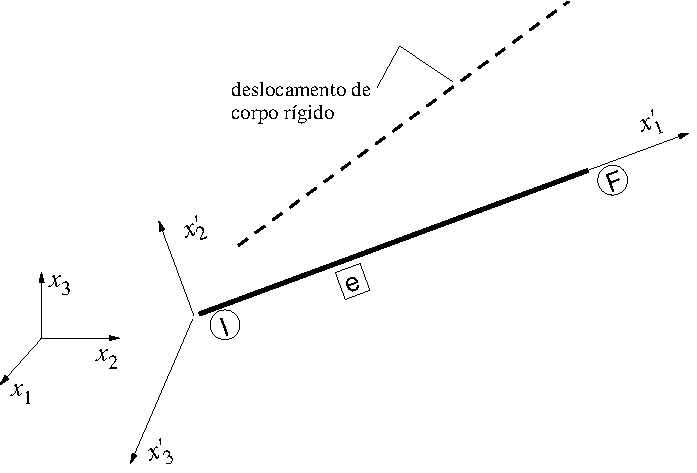
\includegraphics[scale=0.6]{img/desl_rig}
		      \captionof{figure}{Elemento sob deslocamento de corpo rígido}
		      \label{deslrig}
		      \vspace{12pt}
	      \end{minipage}

\end{enumerate}

\section{Sistema de Equações de Equilíbrio}

Suponha que um sistema estrutural componha-se de \(ne\) elementos e \(nno\) nós, usados na definição dos elementos (de sua incidência). Para detalhamento da estratégia de obtenção do sistema de equações de equilíbrio, considere-se a parte do sistema estrutural reticulado mostrado na Fig. \ref{str1_part}.

\begin{figure}[htb!]
	\begin{subfigure}{0.49\textwidth}
		\begin{center}
			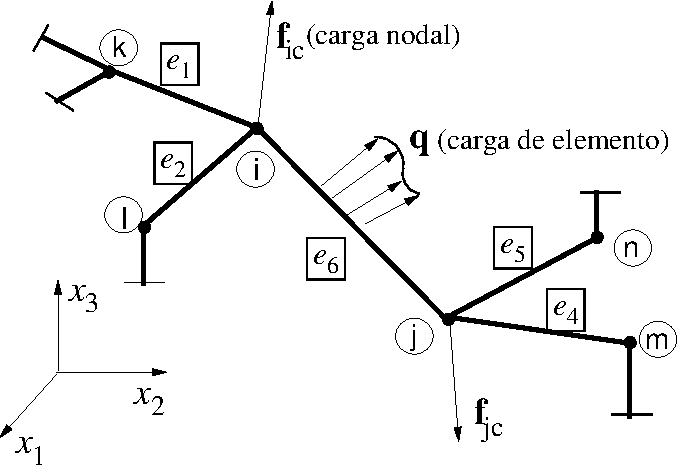
\includegraphics[scale=0.55]{img/struct-p1}
			\caption{\footnotesize Corte em vários elementos}
			\label{corte_str1}   \vspace{12pt}
		\end{center}
	\end{subfigure}
	\begin{subfigure}{0.49\textwidth}
		\begin{center}
			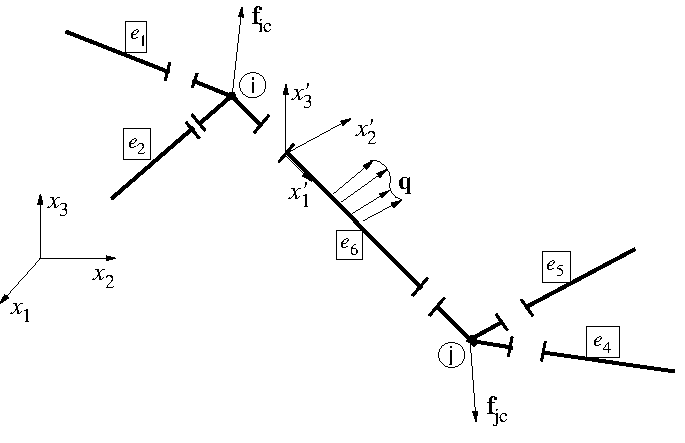
\includegraphics[scale=0.6]{img/struct-el1}
			\caption{\footnotesize Detalhe em elemento}
			\label{corte_el2}   \vspace{12pt}
		\end{center}
	\end{subfigure}
	\caption{Corte de parte da estrutura.}
	\label{str1_part}
\end{figure}

Estabelecendo-se que o nó inicial do elemento \(e_6\) seja o nó \(i\) e o final, o nó \(j\), obtém-se para esse elemento o referencial local S' indicado na Fig. \ref{corte_el2}, no qual \(x'_1\) tem a direção do eixo do elemento e \(x'_2\) e \(x'_3\) não são necessariamente eixos principais da seção. Definidos os eixos de elemento, a matriz de rotação do elemento, \(\mathbf{R^{(e_6)}}\), pode então ser diretamente calculada, de modo que dispondo-se da matriz de rigidez local de elemento, a correspondente matriz global pode ser obtida. Para a carga de elemento \(\mathbf{q}\), as respectivas ações nodais equivalentes, locais e globais, podem também ser obtidas. Neste elemento da estrutura, atuará portanto, ao final (ou seja, após a estrutura ter atingido o equilíbrio), as ações mostradas na representação gráfica da Fig. \ref{el_forces}, onde

\begin{minipage}{0.35\textwidth}
	\(\mathbf{f_{i0}^{'(e_6)}}\) e \(\mathbf{f_{j0}^{'(e_6)}}\) são as ações locais de engastamento perfeito para o agente externo solicitante (reações de viga biengastada para \(\mathbf{q}\)).

	\

	\(\mathbf{a_{i}^{'(e_6)}}\) e \(\mathbf{a_{j}^{'(e_6)}}\) são as ações locais de extremidade de elemento em função de seus deslocamentos nodais.
\end{minipage}
\begin{minipage}{0.6\textwidth}
	\begin{center}
		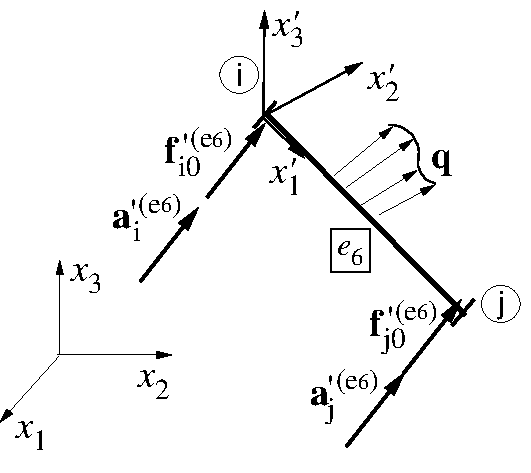
\includegraphics[scale=0.6]{img/struct-el2}
		\captionof{figure}{Forças de elemento}
		\label{el_forces}   \vspace{12pt}
	\end{center}
\end{minipage}

Na verdade, o sistema global de equações do método da rigidez direta (baseado em deslocamentos) é obtido impondo-se a condição de equilíbrio (de ações) a todos os nós do modelo. Considerando-se, por exemplo, o nó \(i\) da estrutura, tem-se, exprimindo-se todas as ações em questão em relação ao referencial global:

\

\begin{minipage}{0.4\textwidth}
	\begin{equation}
		\label{eq:1}
		\mathbf{f}_{ic} - \sum\limits_{j=1}^{nei}\mathbf{f}_{i0}^{(e_{ji})}- \sum\limits_{j=1}^{nei}\mathbf{a}_{i}^{(e_{ji})}=\mathbf{0}
	\end{equation}
\end{minipage}
\begin{minipage}{0.55\textwidth}
	\begin{center} %	\hspace{1,5cm}
		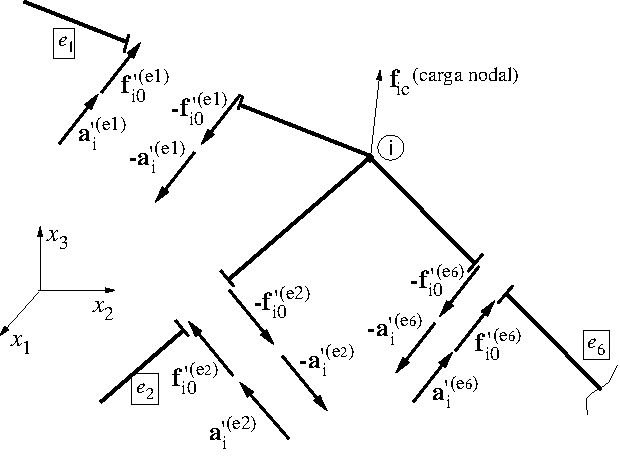
\includegraphics[scale=0.6]{img/struct-node}
		\captionof{figure}{Forças no nó \textit{i}.}
		\label{node_forces}   \vspace{12pt}
	\end{center}
\end{minipage}

\noindent onde \(nei\) é o número de elementos que concorrem no nó \(i\) e \(e_{ji}\) denota a numeração do j-ésimo elemento que nele concorre. Considerando-se ainda que as conectividades de \(e_1\) e \(e_2\) sejam dadas conforme Tabela \ref{conect}, tem-se:
\begin{table}[htb!]
	\centering
	\caption{Conectividades de \(e_1\) e \(e_2\)}	\label{conect}
	\begin{tabular}{c|c}
		nó inicial     & nó final       \\  \hline
		\(noi(e_1)=k\) & \(nof(e_1)=i\) \\ %\hline
		\(noi(e_2)=i\) & \(nof(e_2)=l\)
	\end{tabular}
\end{table}
\begin{align}
	\label{eq:2}
	\nonumber \mathbf{a}_{i}^{(e_{1})}=\mathbf{k}_{ik}^{(e_{1})} \cdot \mathbf{u}_{k}^{(e_{1})} + \mathbf{k}_{ii}^{(e_{1})} \cdot \mathbf{u}_{i}^{(e_{1})} \\
	\mathbf{a}_{i}^{(e_{2})}=\mathbf{k}_{ii}^{(e_{2})} \cdot \mathbf{u}_{i}^{(e_{2})} + \mathbf{k}_{il}^{(e_{2})} \cdot \mathbf{u}_{l}^{(e_{2})}           \\
	\nonumber \mathbf{a}_{i}^{(e_{6})}=\mathbf{k}_{ii}^{(e_{6})} \cdot \mathbf{u}_{i}^{(e_{6})} + \mathbf{k}_{ij}^{(e_{6})} \cdot \mathbf{u}_{j}^{(e_{6})}
\end{align}
\noindent onde os subscritos nestas expressões (\(i,k,j\)) agora denotam a numeração global dos nós envolvidos. Substituindo-se então \eqref{eq:2} em \eqref{eq:1} obtém-se:

\begin{align}
	\sum\limits_{j=1}^{nei}\mathbf{a}_{i}^{(e_{ji})}
	 & = \mathbf{a}_{i}^{(e_{1})}+\mathbf{a}_{i}^{(e_{2})}+\mathbf{a}_{i}^{(e_{6})} \nonumber                                                                                                                                                                                                                                                 \\
	 & = \mathbf{k}_{ik}^{(e_{1})} \cdot \mathbf{u}_{k}^{(e_{1})} + \mathbf{k}_{ii}^{(e_{1})} \cdot \mathbf{u}_{i}^{(e_{1})} + \mathbf{k}_{ii}^{(e_{2})} \cdot \mathbf{u}_{i}^{(e_{2})} + \mathbf{k}_{il}^{(e_{2})} \cdot \mathbf{u}_{l}^{(e_{2})} +\mathbf{k}_{ii}^{(e_{6})} \cdot \mathbf{u}_{i}^{(e_{6})} + \mathbf{k}_{ij}^{(e_{6})} \cdot \mathbf{u}_{j}^{(e_{6})} \nonumber \\
	 & = \mathbf{f}_{ic} - \left [ \mathbf{f}_{i0}^{(e_{1})}+\mathbf{f}_{i0}^{(e_{2})}+\mathbf{f}_{i0}^{(e_{6})}\right ]
\end{align}

\noindent Admitindo-se que o nó \(i\) seja rígido, que não haja portanto qualquer descontinuidade de deslocamento, como rótulas, por exemplo, tem-se que:

\[ \mathbf{u}_{i}^{(e_{1})}=\mathbf{u}_{i}^{(e_{2})}=\mathbf{u}_{i}^{(e_{6})}=\mathbf{u}_{i}\]

\noindent e a equação de equilíbrio para o nó \(i\) fica então:

\[\mathbf{k}_{ik}^{(e_{1})} \cdot \mathbf{u}_{k}^{(e_{1})} + \left [ \mathbf{k}_{ii}^{(e_{1})}+\mathbf{k}_{ii}^{(e_{2})}+\mathbf{k}_{ii}^{(e_{6})}\right ]\cdot \mathbf{u_{i}}+ \mathbf{k}_{il}^{(e_{2})} \cdot \mathbf{u}_{l}^{(e_{2})} + \mathbf{k}_{ij}^{(e_{6})} \cdot \mathbf{u}_{j}^{(e_{6})}=\mathbf{f}_{ic} - \left [ \mathbf{f}_{i0}^{(e_{1})}+\mathbf{f}_{i0}^{(e_{2})}+\mathbf{f}_{i0}^{(e_{6})}\right ] \]

ou ainda,

\[ \mathbf{k}_{ii}\cdot \mathbf{u}_i + \mathbf{k}_{ij}^{(e_{6})} \cdot \mathbf{u}_{j}^{(e_{6})} + \mathbf{k}_{ik}^{(e_{1})} \cdot \mathbf{u}_{k}^{(e_{1})} + \mathbf{k}_{il}^{(e_{2})} \cdot \mathbf{u}_{l}^{(e_{2})} = \mathbf{f}_i \]

com,
\[\mathbf{k}_{ii}=\sum\limits_{j=1}^{nei}\mathbf{k}_{ii}^{(e_{ji})}\]

\[\mathbf{f}_i=\mathbf{f}_{ic} - \sum\limits_{j=1}^{nei}\mathbf{f}_{i0}^{(e_{ji})}\]

\

Considerando-se agora o nó \(j\) e imaginando-se que as conectividades de \(e_4\) e \(e_5\) sejam dadas na Tabela \ref{conect_eJ}, tem-se, procedendo-se de forma análoga:
\begin{table}[htb!]
	\centering
	\caption{Conectividades de \(e_4\) e \(e_5\)}	\label{conect_eJ}
	\begin{tabular}{c|c}
		nó inicial     & nó final       \\  \hline
		\(noi(e_4)=j\) & \(nof(e_4)=m\) \\ %\hline
		\(noi(e_5)=j\) & \(nof(e_5)=n\)
	\end{tabular}
\end{table}
\begin{align*}
	\sum\limits_{k=1}^{nej}\mathbf{a}_{j}^{(e_{kj})} & = & \mathbf{a}_{j}^{(e_{4})}+\mathbf{a}_{j}^{(e_{5})}+\mathbf{a}_{j}^{(e_{6})} \nonumber                                                                                                                                                                                                                                                 \\
	                                             & = & \mathbf{k}_{jj}^{(e_{4})} \cdot \mathbf{u}_{j}^{(e_{4})} + \mathbf{k}_{jm}^{(e_{4})} \cdot \mathbf{u}_{m}^{(e_{4})} + \mathbf{k}_{jj}^{(e_{5})} \cdot \mathbf{u}_{j}^{(e_{5})} + \mathbf{k}_{jn}^{(e_{5})} \cdot \mathbf{u}_{n}^{(e_{5})} +\mathbf{k}_{ji}^{(e_{6})} \cdot \mathbf{u}_{i}^{(e_{6})} + \mathbf{k}_{jj}^{(e_{6})} \cdot \mathbf{u}_{j}^{(e_{6})} \nonumber \\
	                                             & = & \mathbf{f}_{jc} - \left [ \mathbf{f}_{j0}^{(e_{4})}+\mathbf{f}_{j0}^{(e_{5})}+\mathbf{f}_{j0}^{(e_{6})}\right ]  \; .
\end{align*}

\noindent Admitindo-se igualmente que \(\mathbf{u}_{j}^{(e_{4})}=\mathbf{u}_{j}^{(e_{5})}=\mathbf{u}_{j}^{(e_{6})}=\mathbf{u}_{j}\) (condição de nó rígido), resulta:

\[\mathbf{k}_{ji}^{(e_{6})} \cdot \mathbf{u}_{i}^{(e_{6})} +\mathbf{k}_{jj}\cdot \mathbf{u}_j + \mathbf{k}_{jm}^{(e_{4})} \cdot \mathbf{u}_{m}^{(e_{4})} + \mathbf{k}_{jn}^{(e_{5})} \cdot \mathbf{u}_{n}^{(e_{5})} = \mathbf{f}_j \]

\noindent com

\[\mathbf{k}_{jj}=\sum\limits_{k=1}^{nej}\mathbf{k}_{jj}^{(e_{kj})}, \quad \mathbf{f}_j=\mathbf{f}_{jc} - \sum\limits_{k=1}^{nej}\mathbf{f}_{j0}^{(e_{kj})}\; . \]

\noindent Alocando-se as equações de equilíbrio para on nós  \(i\) e \(j\) no sistema de equações global de toda a estrutura, que contém as equações de equilíbrio de todos os nós, tem-se:
\pagebreak
\begin{figure}[!ht]
	\begin{center} %\hspace{-1,0cm}
		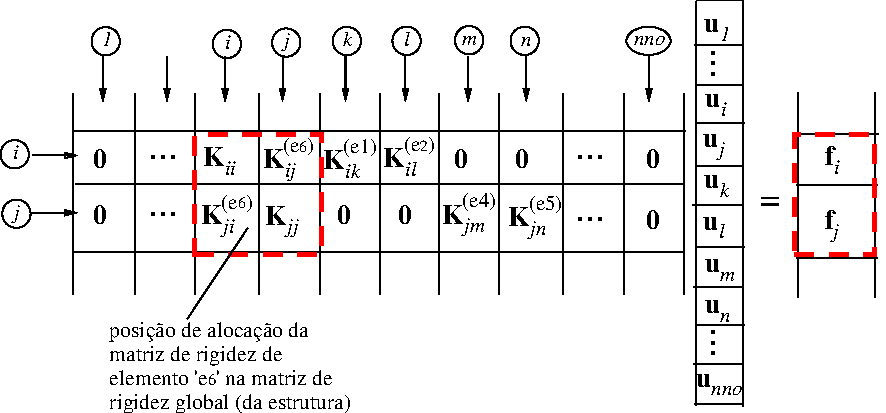
\includegraphics[scale=0.9]{img/gl_syst1}
		\captionof{figure}{Alocação de \(\mathbf{K}^{(e_k)}_{ij}\) em \(\mathbf{K}\) (matriz de rigidez global)}
		\label{corte_el1}   \vspace{12pt}
	\end{center}
\end{figure}

\noindent ou de forma compacta, após a inclusão das equações de equilíbrio para os outros nós,

\[ \mathbf{K\cdot u}=\mathbf{f}  \; ,\]

\noindent onde \(\mathbf{K}\) é a matriz de rigidez global do sistema estrutural, \(\mathbf{u}\) é o vetor de deslocamentos nodais globais e \(\mathbf{u}\), o vetor de cargas nodais equivalentes.

\medskip

\noindent Observações:
\begin{enumerate}

	\item  Como vê-se do detalhamento da estratégia de obtenção do sistema de equações, pode-se de um modo geral calcular a matriz de rigidez global de cada elemento e alocá-la na matriz global da estrutura em função das conectividades do elemento, ou seja, pode-se adotar o seguinte esquema de montagem:

	      do i=1,ne

	      - cálculo de \(\mathbf{K}^{(ei)}\)

	      - alocação de \(\mathbf{K}^{(ei)}\) em \(\mathbf{k}\)

	      end do

	\item  Para o vetor de cargas, \(\mathbf{f}\), dado o nó em que há carga (concentrada ou advinda de carga de elemento), seu valor é diretamente alocado em função de sua numeração global.

	      \medskip

	\item  Dado que as matrizes de rigidez de estruturas em geral são usualmente esparsas, ou seja, contêm muitos blocos de nulos, é conveniente usar formatos de armazenamento, como por exemplo, em banda ou em perfil (skyline), através dos quais o armazenamento e processamento de tais blocos sejam minimizados.
\end{enumerate}
\

A alocação (espalhamento) da matriz de rigidez do elemento \(e\), \(\mathbf{K}^{(e)}\), e do vetor de cargas nodais equivalentes, referenciados aos eixos globais, na matriz de rigidez e correspondente vetor de cargas da estrutura é esboçada na Fig. \ref{gldof_el}, onde se indica a determinação da numeração global dos graus de liberdade do elemento \(e\).
\clearpage
\begin{figure}[tbh!]
	\begin{center}
		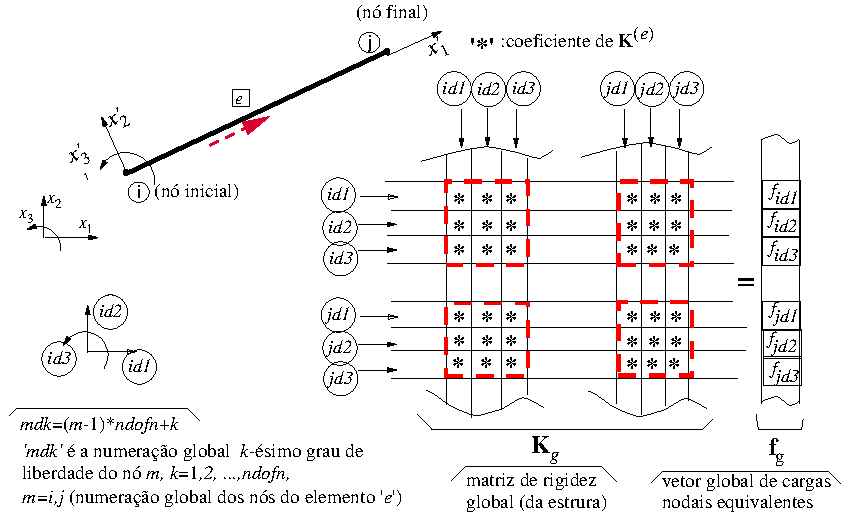
\includegraphics[scale=0.9]{img/aloc1}
		\caption{Numeração global dos graus de liberdade associados ao elemento \(e\)}
		\label{gldof_el}
		\vspace{12pt}
	\end{center}
\end{figure}

\section{Descontinuidades de deslocamentos  entre elementos}

Entre elementos estruturais reticulados, poderá haver descontinuidades que impossibilitem a transmissão dos demais tipos de esforços simples entre elementos (vide modelos na Fig. \ref{descnt1}). Neste caso, faz-se necessário simular a correspondente descontinuidade de deslocamento. Para isso, como vê-se das equações de equilíbrio nodal mostradas anteriormente, basta não superpor os coeficientes de rigidez de elementos associados aos graus de liberdade em que haja descontinuidade. Note-se que a superposição de coeficientes em formulações baseadas em deslocamentos corresponde à imposição de continuidade entre os respectivos graus de liberdade dos elementos em questão.

\begin{figure}[tbh!]
	\begin{center} %\hspace{-1,0cm}
		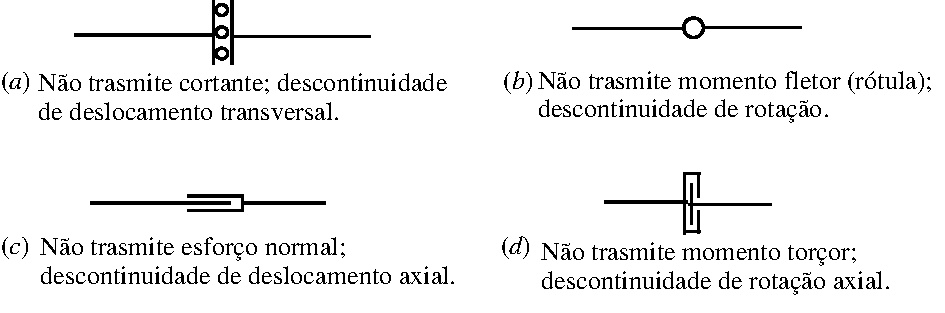
\includegraphics[scale=0.9]{img/descont1}
		\caption{Tipos de descontinuidades entre elementos}
		\label{descnt1}   \vspace{12pt}
	\end{center}
\end{figure}

Assim, para o nó rotulado de pórtico plano indicado na Fig. \ref{rot1}, escrevem-se as seguintes de equações de equilíbrio para o nó \(i\):
\begin{equation} \label{rot_eq}
	\left\{ \begin{array}{l}
		\sum F_{x_1}=f_{i_1}^{(e_1,e_2,e_3)}-[ a_{i_1}^{(e_1)}+a_{i_1}^{(e_2)}+a_{i_1}^{(e_3)} ]=0 \\
		\sum F_{x_2}=f_{i_2}^{(e_1,e_2,e_3)}-[ a_{i_2}^{(e_1)}+a_{i_2}^{(e_2)}+a_{i_2}^{(e_3)} ]=0 \\
		\sum F_{x_3}^{(e_1,e_3)}=f_{i_3}^{(e_1,e_3)}-[ a_{i_3}^{(e_1)}+a_{i_3}^{(e_3)} ]=0         \\
		\sum F_{x_3}^{(e_2)}=f_{i_3}^{(e_2)}-a_{i_3}^{(e_2)}=0
	\end{array}
	\right.
\end{equation}
\begin{figure}[tbh!]
	\begin{center} %\hspace{-1,0cm}
		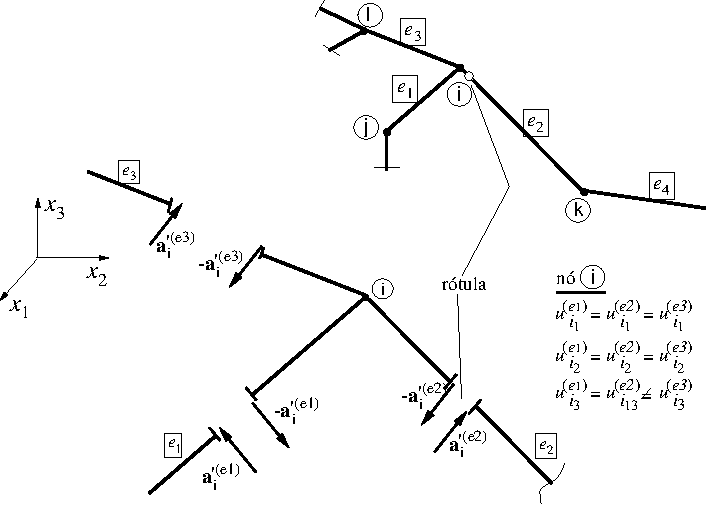
\includegraphics[scale=0.9]{img/rotula1}
		\caption{Rótula no nó \(i\) pelo elemento \(e_2\)}
		\label{rot1}   \vspace{12pt}
	\end{center}
\end{figure}

\noindent \underline{Observação}: \vspace{6pt}

\noindent Note-se que como os graus de liberdade dos elementos são desacoplados segundo a direção \(x_3\), então as equações de equilíbrio de ações nessa direção são independentes; por isso há duas equações de equilíbrio. Em geral, haverá \((n+1)\) equação de equilíbrio, onde \(n\) é o número de elementos que se conectem rotuladamente a um nó.

\

Particionando-se a submatriz de rigidez \(\mathbf{K}_{ij}^{(e)}\) (associada aos nós \(i\) e \(j\) de um certo elemento \(e\)) nas formas

\[\mathbf{K}_{ij}^{(e)}=\left[ \mathbf{k}_{ij_1}^{(e)} \quad \mathbf{k}_{ij_2}^{(e)} \quad  \mathbf{k}_{ij_3}^{(e)} \right] \;\; \textrm{(por colunas)}, \quad
	\mathbf{K}_{ij}^{(e)}= \left[\;\; \begin{matrix}
			\mathbf{k}_{i_1j}^{(e)}  \vspace{5pt} \\
			\mathbf{k}_{i_2j}^{(e)} \vspace{5pt}  \\
			\mathbf{k}_{i_3j}^{(e)}
		\end{matrix} \right]   \textrm{(por linhas)}, \]

\noindent onde \(i_m\) denota o \(m\)-ésimo grau de liberdade do nó \(i\), pode-se então escrever:

\begin{equation} \left\{ \begin{array}{l}\label{intf1}
		\mathbf{a}_{i}^{(e_1)}=\mathbf{k}_{ii_1}^{(e_1)}{u}_{i_1}^{(e_1)}+\mathbf{k}_{ii_2}^{(e_1)}{u}_{i_2}^{(e_1)}+\mathbf{k}_{ii_3}^{(e_1)}{u}_{i_3}^{(e_1)}+\mathbf{k}_{ij}^{(e_1)}\mathbf{u}_{j}^{(e_1)} \vspace{5pt} \\
		\mathbf{a}_{i}^{(e_2)}=\mathbf{k}_{ii_1}^{(e_2)}u_{i_1}^{(e_2)}+\mathbf{k}_{ii_2}^{(e_2)}u_{i_2}^{(e_2)}+\mathbf{k}_{ii_3}^{(e_2)}u_{i_3}^{(e_2)}+\mathbf{K}_{ik}^{(e_2)}\mathbf{u}_{k}^{(e_2)} \vspace{5pt}       \\
		\mathbf{a}_{i}^{(e_3)}=\mathbf{k}_{ii_1}^{(e_3)}u_{i_1}^{(e_3)}+\mathbf{k}_{ii_2}^{(e_3)}u_{i_2}^{(e_3)}+\mathbf{k}_{ii_3}^{(e_3)}u_{i_3}^{(e_3)}+\mathbf{k}_{il}^{(e_3)}\mathbf{u}_{l}^{(e_3)}
	\end{array}  \right. \;.
\end{equation}

\noindent Considerando-se as relações entre os deslocamentos do nó \(i\) dadas na Fig.  \ref{rot1} e fazendo-se

\begin{equation} \left\{ \begin{array}{l}u_{i_m}^{(e_1)}=u_{i_m}^{(e_2)}=u_{i_m}^{(e_3)}=u_{i_m}, \; m=1,2, \quad  u_{i3}^{(e_1)}=u_{i_3}^{(e_3)}\neq u_{i_3}^{(e_2)}  \vspace{5pt} \\
		\mathbf{u}_{j}^{(e_1)}=\mathbf{u}_j, \quad  \mathbf{u}_{k}^{(e_2)}=\mathbf{u}_k , \quad \mathbf{u}_{l}^{(e_3)}=\mathbf{u}_l
	\end{array} \right. \; ,
\end{equation}
\noindent vê-se que as equações de equilíbrio para o nó \(i\) são da forma:
\begin{multline}\label{eq_rot1} \scalebox{0.85}{$
			\left[\begin{array}{cc:cc:ccc}
					\left( k_{i_1 i_1}^{(e_1)}+k_{i_1 i_1}^{(e_2)}+k_{i_1 i_1}^{(e_3)} \right) & \left( k_{i_1 i_2}^{(e_1)}+k_{i_1 i_2}^{(e_2)}+k_{i_1 i_2}^{(e_3)} \right) &
					\left( k_{i_1 i_3}^{(e_1)}+k_{i_1 i_3}^{(e_3)} \right)                     & k_{i_1 i_3}^{(e_2)}                                                        & \mathbf{k}_{i_1 j}^{(e_1)} & \mathbf{k}_{i_1 k}^{(e_2)} & \mathbf{k}_{i_1 l}^{(e_3)} \\
					\left( k_{i_2 i_1}^{(e_1)}+k_{i_2 i_1}^{(e_2)}+k_{i_2 i_1}^{(e_3)} \right) & \left( k_{i_2 i_2}^{(e_1)}+k_{i_2 i_2}^{(e_2)}+k_{i_2 i_2}^{(e_3)} \right) &
					\left( k_{i_2 i_3}^{(e_1)}+k_{i_2 i_3}^{(e_3)} \right)                     & k_{i_2 i_3}^{(e_2)}                                                        & \mathbf{k}_{i_2 j}^{(e_1)} & \mathbf{k}_{i_2 k}^{(e_2)} & \mathbf{k}_{i_2 l}^{(e_3)} \\ \hdashline[8pt/2pt]
					\left( k_{i_3 i_1}^{(e_1)}+k_{i_3 i_1}^{(e_3)} \right)                     & \left( K_{i_3 i_2}^{(e_1)}+k_{i_3 i_2}^{(e_3)} \right)                     &
					\left( k_{i_3 i_3}^{(e_1)}+k_{i_3 i_3}^{(e_3)} \right)                     & 0                                                                          & \mathbf{k}_{i_3 j}^{(e_1)} & 0                      & \mathbf{k}_{i_3 l}^{(e_3)} \\
					k_{i_3 i_1}^{(e_2)}                                                        & k_{i_3 i_2}^{(e_2)}                                                        &
					0                                                                          & k_{i_3 i_3}^{(e_2)}                                                        & \mathbf{0}                 & \mathbf{k}_{i_3 k}^{(e_2)} & \mathbf{0}\end{array} \right]  $}
	\cdot \left\{ \begin{array}{c}
		u_{i_1} \\ u_{i_2} \\ \hdashline[8pt/2pt]   u_{i_3}^{(e_1)} \\ u_{i_3}^{(e_2)} \\  \hdashline[8pt/2pt]  \mathbf{u}_{j}  \\ \mathbf{u}_{k} \\ \mathbf{u}_{l}\end{array}   \right\} \\
	= \left\{ \begin{array}{c}
		f_{i_1}^{(e_1,e_2,e_3)} \vspace{5pt} \\ f_{i_2}^{(e_1,e_2,e_3)} \vspace{5pt} \\\hdashline[8pt/2pt]  f_{i_3}^{(e_1,e_3)} \vspace{5pt} \\ f_{i_3}^{(e_2)} \\\hdashline[8pt/2pt]\end{array} \right\} \quad \quad
\end{multline}

\noindent Observações:
\begin{enumerate}
	\item Note que a não-superposição das colunas associadas ao grau de liberdade \(i_3\) corresponde à simulação de descontinuidade de deslocamento, enquanto a não-superposição das linhas relaciona-se com o fato de que as equações de equilíbrio de ação nessa direção são independentes.

	\item Na Fig. \ref{port1}, indica-se um pórtico rotulado e o correspondente aspecto de sua matriz de rigidez conforme o processo de consideração de descontinuidade descrito acima.

	      \begin{figure}[tbh!]
		      \begin{center}
			      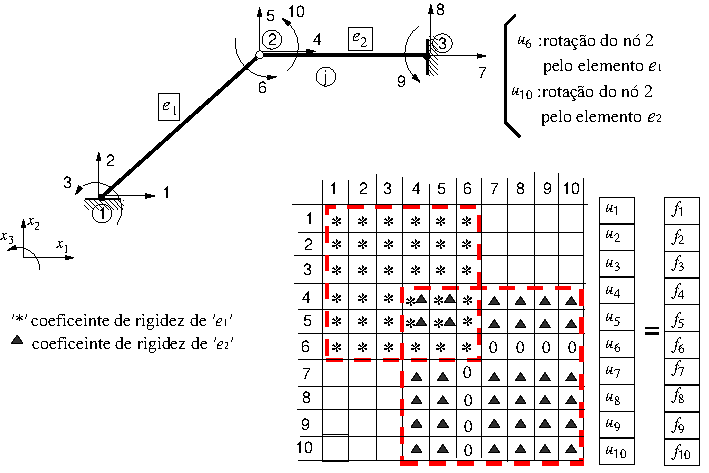
\includegraphics[scale=1.2]{img/port_rot1}
			      \caption{Matriz de rigidez (aspecto) de pórtico rotulado} \label{port1}
		      \end{center}
	      \end{figure}

	\item  O processo é geral e se aplica na simulação de qualquer tipo de descontinuidade de qualquer tipo de elemento.

	\item O processo é extremamente útil para o desenvolvimento de códigos computacionais para análise inelástica, uma vez que a plastificação de uma seção nada mais é do que uma descontinuidade de elemento.

	\item Escrevendo-se o conjunto de equações de equilíbrio para \(k\), obtém-se (vide img. \ref{rot1} e \ref{nok}):
	      \[ \left[ \begin{matrix} \;\;
				      \mathbf{K}_{ki_1}^{(e_2)} & \mathbf{K}_{ki_2}^{(e_2)} & \mathbf{0} & \mathbf{K}_{ki_3}^{(e_2)} & \mathbf{0} & \left( \mathbf{K}_{kk}^{(e_2)} + \mathbf{K}_{kk}^{(e_4)}\right) & \mathbf{0} & \mathbf{K}_{km}^{(e_4)}
			      \end{matrix} \right] \left[ \;\;\begin{matrix}
				      u_{i_1} \\ u_{i_2} \\ u_{i_3}^{(e_1)} \\ u_{i_3}^{(e_2)} \\ \mathbf{u}_{j} \\ \mathbf{u}_{k} \\ \mathbf{u}_{l} \\ \mathbf{u}_{m}
			      \end{matrix} \right] = \left[ \mathbf{f}_k \right] \]
	      \begin{figure}[tbh!]
		      \begin{center} %\hspace{-1,0cm}
			      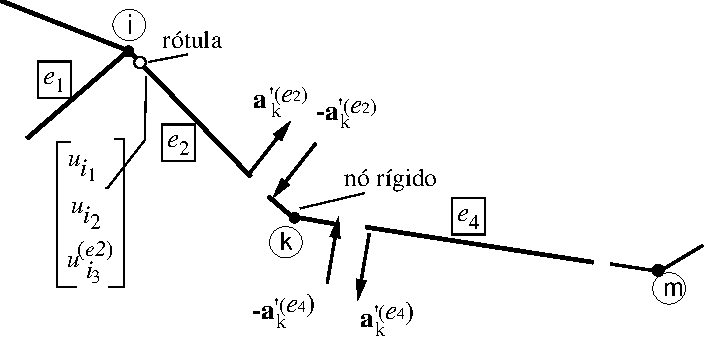
\includegraphics[scale=0.9]{img/port_nok}
			      \caption{Equilíbrio do nó \(k\)} \label{nok}
		      \end{center}
	      \end{figure}

\end{enumerate}

Alternativamente, matrizes de rigidez de elemento podem ser obtidas de modo a diretamente simular suas descontinuidades. Para isso, condensam-se os graus de liberdade correspondentes às descontinuidades, \(\mathbf{u}_l\), nos outros graus de liberdades. Em geral, tem-se:

\begin{equation} \mathbf{K}\mathbf{u}=\left[\;\; \begin{matrix}
			\mathbf{K}_{00} & \mathbf{K}_{0l} \\
			\mathbf{K}_{l0} & \mathbf{K}_{ll}
		\end{matrix} \right] \left[\;\; \begin{matrix}
			\mathbf{u}_{0} \\ \mathbf{u}_{l}
		\end{matrix} \right] = \left\{ \;\; \begin{matrix}
		\mathbf{K}_{00}\mathbf{u}_{0} + \mathbf{K}_{0l}\mathbf{u}_{l} = \mathbf{a}_0 \\
		\mathbf{K}_{l0}\mathbf{u}_{0} + \mathbf{K}_{ll}\mathbf{u}_{l} = \mathbf{a}_l   \label{part_ke}
	\end{matrix} \right.\end{equation}

\noindent Da 2ª equação do sistema (\ref{part_ke}), tem-se:

\begin{equation} \label{ufree}
	\mathbf{K}_{ll}\mathbf{u}_{l} = \mathbf{a}_l - \mathbf{K}_{l0}\mathbf{u}_{0} ; \quad \mathbf{u}_{l} = \mathbf{K}_{ll}^{-1}\mathbf{a}_l - \mathbf{K}_{ll}^{-1}\mathbf{K}_{l0}\mathbf{u}_{0} \; .
\end{equation}
Substituindo-se \(\mathbf{u}_{l}\) na 1ª equação do sistema, resulta:
\begin{align*}
	\mathbf{K}_{00}\mathbf{u}_{0}   + \mathbf{K}_{0l}\left( \mathbf{K}_{ll}^{-1}\mathbf{a}_l - \mathbf{K}_{ll}^{-1}\mathbf{K}_{l0}\mathbf{u}_{0} \right) & =  \left(\mathbf{K}_{00} - \mathbf{K}_{0l}\mathbf{K}_{ll}^{-1}\mathbf{K}_{l0}\right)\mathbf{u}_{0} + \mathbf{K}_{0l}\mathbf{K}_{ll}^{-1}\mathbf{a}_l = \bf{a}_0  \, ; \\
	\left(\mathbf{K}_{00} - \mathbf{K}_{0l}\mathbf{K}_{ll}^{-1}\mathbf{K}_{l0}\right)\mathbf{u}_{0}                                          & = \mathbf{a}_0 - \mathbf{K}_{0l}\mathbf{K}_{ll}^{-1}\mathbf{a}_l\end{align*}
Considerando que \(\mathbf{a}_l=\mathbf{0}\), já que não há transmissão de esforços via graus de liberdade correspondentes às descontinuidades do elemento, obtém-se:
\[ \mathbf{K}_{00}^{(d)}\mathbf{u}_{0} = \mathbf{a}_0 , \quad \textrm{com}\quad \mathbf{K}_{00}^{(d)} = \mathbf{K}_{00} - \mathbf{K}_{0l}\mathbf{K}_{ll}^{-1}\mathbf{K}_{l0} \; .\]
Por exemplo, para o cálculo da matriz de elemento de pórtico plano com rótula na direção do grau de liberdade \(6\), mostrado na Fig. \ref{el_rot1}, tem-se
\begin{figure}[tbh!]
	\begin{center} %\hspace{-1,0cm}
		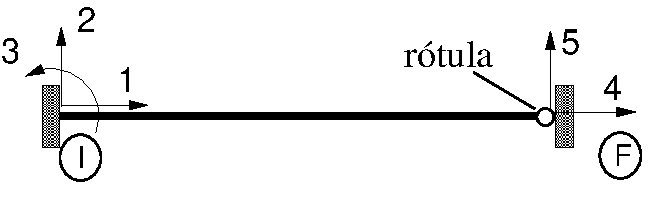
\includegraphics[scale=0.6]{img/el_rotula1}
		\caption{Elemento de pórtico plano rotulado (com \(5\) graus de liberdade)} \label{el_rot1}
	\end{center}
\end{figure}
\begin{equation} \mathbf{K}_{00}^{(d)}=\left[ \; \begin{array}{ccccc}
			k_{11} & k_{12} & k_{13} & k_{14} & k_{15} \\
			k_{21} & k_{22} & k_{23} & k_{24} & k_{25} \\
			k_{31} & k_{32} & k_{33} & k_{34} & k_{35} \\
			k_{41} & k_{42} & k_{43} & k_{44} & k_{45} \\
			k_{51} & k_{52} & k_{53} & k_{54} & k_{55}
		\end{array} \right] - \left[ \;\begin{array}{c}
			k_{16} \\ k_{26} \\ k_{36} \\ k_{46} \\ k_{56}
		\end{array} \right]\! \cdot \! \left(\frac{1}{k_{66}} \right) \! \cdot \!
	\left[ \; \begin{array}{ccccc} k_{61} & k_{62} & k_{63} & k_{64} & k_{65}
		\end{array} \right] \; . \label{elrot_rig}
\end{equation}

\noindent Sendo
\begin{equation} \mathbf{B}= \mathbf{K}_{0l}\mathbf{K}_{ll}^{-1}\mathbf{K}_{l0}=\frac{1}{k_{66}}\!\cdot\!
	\left[ \; \begin{array}{ccccc}
			k_{16}k_{61} & k_{16}k_{62} & k_{16}k_{63} & k_{16}k_{64} & k_{16}k_{65} \\
			k_{26}k_{61} & k_{26}k_{62} & k_{26}k_{63} & k_{26}k_{64} & k_{26}k_{65} \\
			k_{36}k_{61} & k_{36}k_{62} & k_{36}k_{63} & k_{36}k_{64} & k_{36}k_{65} \\
			k_{46}k_{61} & k_{46}k_{62} & k_{46}k_{63} & k_{46}k_{64} & k_{46}k_{65} \\
			k_{56}k_{61} & k_{56}k_{62} & k_{56}k_{63} & k_{56}k_{64} & k_{56}k_{65}
		\end{array} \right] \; ,\end{equation}
\noindent e considerando que, para pórticos planos, \(k_{12}=k_{13}=k_{15}=k_{16}=k_{24}=k_{34}=k_{45}=k_{46}=0\) e que, da simetria de \(\mathbf{K}\), \(k_{ij}=k_{ji}\), tem-se:
\[ \mathbf{B}=\frac{1}{k_{66}}\!\cdot\!
	\left[ \;\; \begin{matrix}
			0 & 0            & 0            & 0 & 0            \\
			0 & k_{26}K_{62} & k_{26}K_{63} & 0 & k_{26}K_{65} \\
			0 & k_{36}k_{62} & k_{36}k_{63} & 0 & k_{36}k_{65} \\
			0 & 0            & 0            & 0 & 0            \\
			0 & k_{56}k_{62} & k_{56}k_{63} & 0 & k_{56}k_{65} \\
		\end{matrix} \right] \; .\]
\noindent Como \(\mathbf{B}\) é também simétrica, resulta por fim:\[\mathbf{K}_{00}^{(d)}=
	\left[\;\; \begin{matrix}
			k_{11} & 0                                                & 0                                                  & k_{14} & 0                                                 \\
			       & \left(k_{22} -\frac{k_{26}}{k_{66}}k_{62}\right) & \left(k_{23} -\frac{k_{26}}{k_{66}}k_{63}\right)   & 0      & \left(k_{25} -\frac{k_{26}}{k_{66}}k_{65} \right) \\
			       &                                                  & \left( k_{33} -\frac{k_{36}}{k_{66}}k_{63} \right) & 0      & k_{35} -\frac{k_{36}}{k_{66}}k_{65}               \\
			       & \textrm{simétrica}                               &                                                    & k_{44} & 0                                                 \\
			       &                                                  &                                                    &        & \left(k_{55} -\frac{k_{56}}{k_{66}}k_{65} \right) \\
		\end{matrix} \right] \; .\]

\noindent Observações:
\begin{enumerate}
	\item  Para a implementação computacional é conveniente considerar

	      \[ \mathbf{K}^{(d)}=
		      \left[\;\; \begin{matrix}
				      \mathbf{K}_{00}^{(d)} & \mathbf{0} \\
				      \mathbf{0}            & \mathbf{0}
			      \end{matrix} \right]_{ndeel\times ndeel}
	      \]
	      com \(ndeel=ndofn \cdot nnoel\), que corresponde ao número de deslocabilidades por elemento. Note que, assim, \(ndeel\) é o mesmo para todos os elementos da estrutura (com ou sem descontinuidades de deslocamentos).

	\item Caso o elemento rotulado considerado anteriormente tivesse rigidezes axial \(\left( EA_{x'_1}\right)\) e flexional \(\left( EI_{{x'_3}}\right)\) constantes, sua matriz de rigidez de ordem \(ndeel\) (como indicado acima) seria:
	      \begin{figure}[tbh!]
		      \begin{center} %\hspace{-1,0cm}
			      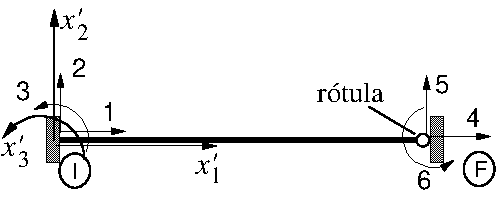
\includegraphics[scale=0.8]{img/el_rotula2}
			      \caption{Elemento de pórtico plano rotulado (com \(6\) graus de liberdade)} \label{el_rot2}
		      \end{center}
	      \end{figure}
	      \[\left\{ \begin{array}{l}
			      k_{11}=-k_{14}=k_{44}=\frac{EA_{x'_1}}{l} ,\vspace{6pt}             \\
			      k_{22}=-k_{25}=k_{55}=\frac{12 EI_{x'_3}}{l^3}, \vspace{6pt}        \\
			      k_{23}=k_{26}=-k_{35}=-k_{56}=\frac{6 EI_{x'_3}}{l^2}, \vspace{6pt} \\
			      k_{33}=k_{66}=\frac{4 EI_{x'_3}}{l}, \quad
			      k_{36}=\frac{2 EI_{x'_3}}{l}\end{array} \right. \;\;,
		      \left\{ \begin{array}{l}
			      k_{11}^{(d)}=k_{11}, \quad k_{22}^{(d)}=\frac{12 EI_{x'_3}}{l^3}-\frac{l}{4EI_{x'_3}}\left( 6\frac{EI_{x'_3}}{l^2} \right)^2=\frac{3 EI_{x'_3}}{l^3}, \vspace{6pt}              \\
			      k_{23}^{(d)}=\frac{6 EI_{x'_3}}{l^2}-\frac{l}{4 EI_{x'_3}}\left( \frac{6 EI_{x'_3}}{l^2} \right)\left( \frac{2 EI_{x'_3}}{l} \right)=\frac{3 EI_{x'_3}}{l^2}, \vspace{6pt}      \\
			      k_{25}^{(d)}=-\frac{12 EI_{x'_3}}{l^3}-\frac{l}{4EI_{x'_3}}\left( \frac{6 EI_{x'_3}}{l^2} \right)\left( -\frac{6 EI_{x'_3}}{l^2} \right)=-\frac{3 EI_{x'_3}}{l^3}, \vspace{6pt} \\
			      k_{33}^{(d)}=\frac{4 EI_{x'_3}}{l}-\frac{l}{4EI_{x'_3}}\left( \frac{2 EI_{x'_3}}{l} \right)^2=\frac{3 EI_{x'_3}}{l}, \vspace{6pt}                                               \\
			      k_{35}^{(d)}=-\frac{6 EI_{x'_3}}{l^2}-\frac{l}{4EI_{x'_3}}\left( 2\frac{EI_{x'_3}}{l} \right)\left( -\frac{6 EI_{x'_3}}{l^2} \right)=-\frac{3 EI_{x'_3}}{l^2}, \vspace{6pt}     \\
			      k_{55}^{(d)}=\frac{12 EI_{x'_3}}{l^3}-\frac{l}{4EI_{x'_3}}\left( -\frac{6 EI_{x'_3}}{l^2} \right)^2=\frac{3 EI_{x'_3}}{l^3}
		      \end{array} \right.  \]

	      \[
		      \mathbf{K}^{(d)}=
		      \left[\;\; \begin{matrix}
				      \frac{EA_{x'}}{l} & 0                    & 0                    & -\frac{EA_{x'}}{l} & 0                     & 0 \\
				                        & 3\frac{EI_{z'}}{l^3} & 3\frac{EI_{z'}}{l^2} & 0                  & -3\frac{EI_{z'}}{l^3} & 0 \\
				                        &                      & 3\frac{EI_{z'}}{l}   & 0                  & -3\frac{EI_{z'}}{l^2} & 0 \\
				                        & \textrm{simétrica}   &                      & \frac{EA_{x'}}{l}  & 0                     & 0 \\
				                        &                      &                      &                    & 3\frac{EI_{z'}}{l^3}  & 0 \\
				                        &                      &                      &                    &                       & 0
			      \end{matrix} \right] \; . \]

	\item  Os zeros nas linhas e colunas associadas aos graus de liberdade em que há descontinuidades exprimem o fato de que as respectivas ações de extremidade de membro (esforços internos decorrentes de deslocamentos que aí haja) não serão computados nas correspondentes equações de equilíbrio.

	\item Na verdade, mais geralmente escreve-se:
	      \[ \left[ \begin{array}{c}
				      \mathbf{a}_0 \\ \mathbf{a}_l
			      \end{array} \right] = \left[ \begin{array}{cc}
				      \mathbf{K}_{00} & \mathbf{K}_{0l} \\ \mathbf{K}_{l0} & \mathbf{K}_{ll}\end{array} \right]\!\cdot\!
		      \left[ \begin{array}{c}
				      \mathbf{u}_0 \\ \mathbf{u}_l
			      \end{array} \right] + \left[ \begin{array}{c}
				      \mathbf{f}_0 \\ \mathbf{f}_l
			      \end{array} \right] \; ,
	      \]
	      \noindent de onde, como anteriormente, tem-se
	      \begin{align*} \mathbf{a}_l & =   \mathbf{K}_{l0}\mathbf{u}_0+ \mathbf{K}_{ll}\mathbf{u}_l + \mathbf{f}_l= \mathbf{0} \; ; \quad \mathbf{u}_l=-\mathbf{K}_{ll}^{-1}\left( \mathbf{K}_{l0}\mathbf{u}_0 + \mathbf{f}_l \right) \; ; \\
	                     \mathbf{a}_0 & =   \mathbf{K}_{00}\mathbf{u}_0+ \mathbf{K}_{0l}\mathbf{u}_l + \mathbf{f}_0=
	                     \mathbf{K}_{00}\mathbf{u}_0- \mathbf{K}_{0l}\mathbf{K}_{ll}^{-1}\left( \mathbf{K}_{l0}\mathbf{u}_0 + \mathbf{f}_l\right) + \mathbf{f}_0                                                            \\
	                              & =  \left( \mathbf{K}_{00}+ \mathbf{K}_{0l}\mathbf{K}_{ll}^{-1}\mathbf{K}_{l0}\right)\mathbf{u}_0 +\left( \mathbf{f}_0-
	                     \mathbf{K}_{0l}\mathbf{K}_{ll}^{-1}\mathbf{f}_l\right) = \mathbf{K}_{00}^{(d)}\mathbf{u}_{0} + \mathbf{f}_0^{(d)} \; ,
	      \end{align*}
	      \noindent com
	      \[\mathbf{K}_{00}^{(d)}=\left( \mathbf{K}_{00}+ \mathbf{K}_{0l}\mathbf{K}_{ll}^{-1}\mathbf{K}_{l0}\right)\; , \quad \mathbf{f}_0^{(d)}= \left( \mathbf{f}_0-
		      \mathbf{K}_{0l}\mathbf{K}_{ll}^{-1}\mathbf{f}_l\right) \; ,
	      \]
	      \noindent sendo \(\mathbf{f}_0\) é o vetor que contém as ações de engastamento perfeito no elemento biengastado, i.e. sem as descontinuidades de deslocamento.

	\item Na implementação computacional para a obtenção das matrizes modificadas, \(\mathbf{K}_{00}^{(d)}\) e \(\mathbf{f}_{0}^{(d)}\), é conveniente, a partir das matrizes de elemento biengastado, \(\mathbf{K}\) e \(\mathbf{f}\), proceder com a liberação dos graus de liberdade desejados, um após após o outro, até a determinação  das matrizes finais \(\mathbf{K}_{00}^{(d)}\) e \(\mathbf{f}_{0}^{(d)}\). Note-se que a ocorrência de uma coeficiente \(k_{jj}\!=\!0\), sem que \(u_j\) seja deslocamento liberado, indica que o conjunto de liberações do elemento conduz a um elemento hipostático.
\end{enumerate}

%Condições de contorno
\section{Condições de Contorno}

Restrições de deslocamento ou deslocamentos prescritos podem ser incluídos no modelo pela estratégia mostrada abaixo. Primeiro, particiona-se o sistema de equações de modo que deslocamentos incógnitos, \(\mathbf{u}_d\), e prescritos, \(\mathbf{u}_r\), sejam agrupados em blocos separados. Tem-se:
\begin{equation} \label{partcc1}
	\left[\;\; \begin{matrix}
			\mathbf{K}_{dd} & \mathbf{K}_{dr} \\
			\mathbf{K}_{rd} & \mathbf{K}_{rr}
		\end{matrix} \right]
	\left[\;\; \begin{matrix}
			\mathbf{u}_{d} \\
			\mathbf{u}_{r}
		\end{matrix} \right] =
	\left[\;\; \begin{matrix}
			\mathbf{f}_{d} \\
			\mathbf{f}_{r}^{(d)}
		\end{matrix} \right] \; .
\end{equation}
Os deslocamentos desconhecidos, \(\mathbf{u}_d\), podem então ser obtidos resolvendo-se
\begin{equation} \label{seq_dis1}
	\mathbf{K}_{dd}\mathbf{u}_{d}=\mathbf{f}_{d}-\mathbf{K}_{dr}\mathbf{u}_{r} \; .
\end{equation}
\noindent Com \(\mathbf{u}_d\), calcula-se então \(\mathbf{f}_{r}^{(d)}\) --- vetor de ações nodais nas direções restringidas decorrentes da deformação estrutural --- por:
\begin{equation} \label{reac0}
	\mathbf{f}_{r}^{(d)}=\mathbf{K}_{rd}\mathbf{u}_{d}+\mathbf{K}_{rr}\mathbf{u}_{r} \; . \end{equation}

Por vezes, o deslocamento em uma certa direção não é diretamente conhecido, porém conhece-se uma relação matemática que descreve a ação nessa direção em função do respectivo deslocamento. Tem-se os chamados apoios elásticos (vide Fig. \ref{apelas}). Neste caso, a ação na direção do apoio elástico precisa ser incluída na equação de equilíbrio na direção do correspondente grau de liberdade.

\begin{figure}[tbh!]
	\begin{center} %\hspace{-1,0cm}
		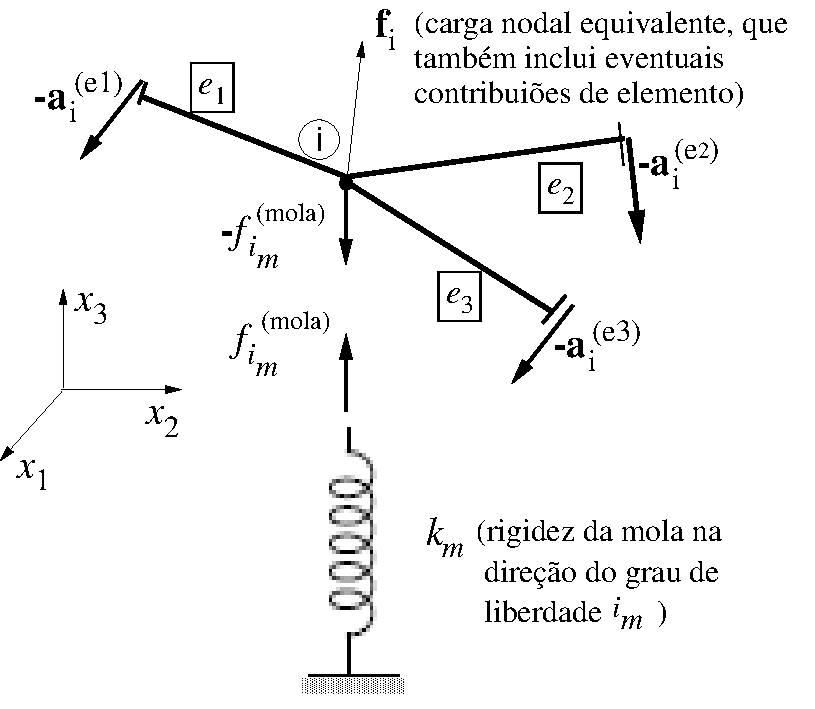
\includegraphics[scale=0.6]{img/apoio_elast1}
		\caption{Apoio elástico na direção do grau de liberdade \(i_m\)} \label{apelas}
	\end{center}
\end{figure}
\noindent Note-se que para deslocamento positivo segundo o \(m\)-ésimo grau de liberdade do nó \(i\), \(i_m\), a correspondente força nodal em \(i\), provocada pela mola, é negativa e dada por: \[f_{i_m}^{(mola)}=-k_m u_{i_m}\; .\]
\noindent Resulta portanto, para essa direção:

\[f_{i_m}-\left( a_{i_m}^{(e_1)} + a_{i_m}^{(e_2)} + a_{i_m}^{(e_3)} \right) - k_m u_{i_m} = f_{i_m} - \sum_{j=1}^{n}k_{i_mj}u_j - k_m u_{i_m}=0  \; ,\]
\noindent ou seja,
\[k_{i_m1}u_1+\cdots +\left( k_{{i_m}{i_m}}+k_m \right)u_{i_m}+\cdots + k_{i_m n}u_n=f_{i_m}, \quad n=\textrm{\textit{nno}}\cdot \textrm{\textit{ndofn}} \;.\]

Alternativamente, os deslocamentos prescritos também podem ser impostos ao sistema estrutural pela técnica de "um e zeros". Neste caso, modifica-se o sistema de equações conforme indica-se abaixo:

\begin{equation} \label{seq_10s}
	\left[\;\; \begin{matrix}
			\mathbf{K}_{dd} & \mathbf{0} \\
			\mathbf{0}      & \mathbf{I}
		\end{matrix} \right]
	\left[ \;\;\begin{matrix}
			\mathbf{u}_{d} \\
			\mathbf{u}
		\end{matrix} \right] =
	\left[\;\; \begin{matrix}
			\mathbf{f}_{d}-\mathbf{K}_{dr}\mathbf{u}_{r} \\
			\mathbf{u}_{r}
		\end{matrix} \right] \end{equation}

Vê-se que, com esta técnica, trabalha-se com um sistema de equações de ordem igual a do sistema inicial, ou seja, não há redução de ordem.

\section{Apoio Inclinado}

Suponha que o suporte em um certo ponto nodal \(i\) seja inclinado (como se mostra na Fig. \ref{apincl}). Como o sistema de equações foi estabelecido em relação ao referencial global, não é possível impor, diretamente, o deslocamento prescrito segundo a direção inclinada \(x'_2\) no nó \(i\).
\begin{figure}[tbh!]
	\begin{center} %\hspace{-1,0cm}
		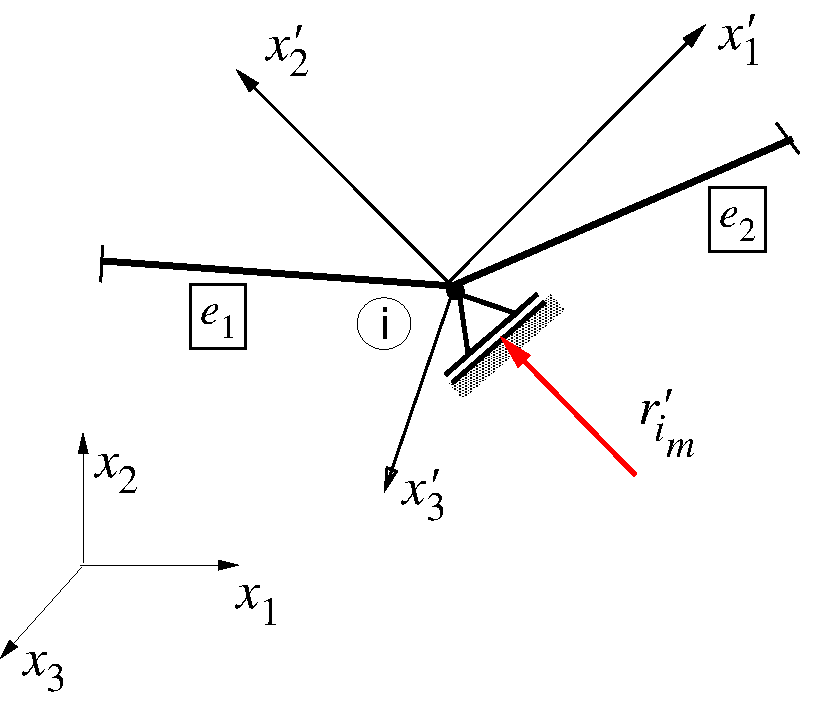
\includegraphics[scale=0.6]{img/apoio_inclinado}
		\caption{Apoio inclinado segundo a direção \(i_m\) do nó \(i\)} \label{apincl}
	\end{center}
\end{figure}
Modificando-se porém o sistema de equações de modo que o vetor de deslocamento do nó \(i\) seja expresso em relação ao referencial local, será então possível prescrever tal condição de contorno. Para isso, procede-se como segue:
\[ {\mathbf{u'}}_i=\mathbf{R}_i \mathbf{u}_i \; ,\qquad {\mathbf{f'}}_i=\mathbf{R}_i \mathbf{f}_i \; ,\]
\noindent onde \(\mathbf{R}_i\) é a transformação de rotação de eixos que converte vetores expressos com relação ao sistema global para o referencial local do apoio inclinado  \(i\). Resulta então:
\begin{align*} \left[\;\; \begin{matrix}
		           \mathbf{K}_{11}u_1                           & \cdots & \left( \mathbf{K}_{1i}\mathbf{R}_i^T \right) \left( \mathbf{R}_i\mathbf{u}_i \right)         & \cdots & \mathbf{K}_{1n}\mathbf{u}_n                      & = & \mathbf{f}_1       \\
		           \vdots                                   & \vdots & \vdots                                                                       & \vdots & \vdots                                   & = & \vdots         \\
		           \left(\mathbf{R}_i\mathbf{K}_{i1}\right)\mathbf{u}_1 & \cdots & \left( \mathbf{R}_i\mathbf{K}_{ii}\mathbf{R}_i^T \right) \left( \mathbf{R}_i\mathbf{u}_i \right) & \cdots & \left(\mathbf{R}_i\mathbf{K}_{in}\right)\mathbf{u}_n & = & \mathbf{R}\mathbf{f}_i \\
		           \vdots                                   & \vdots & \vdots                                                                       & \vdots & \vdots                                   & = & \vdots         \\
		           \mathbf{K}_{i1}\mathbf{u}_1                      & \cdots & \left( \bf{K}_{i}R_i^T \right) \left( \mathbf{R}_i\mathbf{u}_i \right)               & \cdots & \mathbf{K}_{nn}\mathbf{u}_n                      & = & \mathbf{f}_n
	           \end{matrix} \right.\end{align*}

\begin{align}   \label{seq_inc1}
	\left[\;\; \begin{matrix}
			\mathbf{K}_{11}                      & \cdots & \left( \mathbf{K}_{1i}\mathbf{R}_i^T \right)         & \cdots & \mathbf{K}_{1n}                      \\
			\vdots                           & \vdots & \vdots                                       & \vdots & \vdots                           \\
			\left(\mathbf{R}_i\mathbf{K}_{i1}\right) & \cdots & \left( \mathbf{R}_i\mathbf{K}_{ii}\mathbf{R}_i^T \right) & \cdots & \left(\mathbf{R}_i\mathbf{K}_{in}\right) \\
			\vdots                           & \vdots & \vdots                                       & \vdots & \vdots                           \\
			\mathbf{K}_{i1}                      & \cdots & \left( \mathbf{K}_{i}\mathbf{R}_i^T \right)          & \cdots & \mathbf{K}_{nn}
		\end{matrix} \right]
	\left[\;\; \begin{matrix}
			\mathbf{u}_1    \\
			\vdots      \\
			{\mathbf{u'}}_i \\
			\vdots      \\
			\mathbf{u}_n
		\end{matrix} \right]=
	\left[\;\; \begin{matrix}
			\mathbf{f}_1  \\
			\vdots    \\
			\mathbf{f}'_i \\
			\vdots    \\
			\mathbf{f}_n
		\end{matrix} \right]\end{align}

\

Ao sistema (\ref{seq_inc1}) pode-se então impor deslocamento prescrito na direção inclinada.

\section{Reações de Apoio}

Havendo restrições de deslocamento em um apoio, na direção de qualquer dos eixos globais da estrutura, então nessa direção eventualmente surgirá uma força, uma reação de apoio, que terá, naturalmente, para essa direção desse nó, de ser acrescida à correspondente equação de equilíbrio.
\begin{figure}[tbh!]
	\begin{minipage}{0.55\textwidth}
		\centering
		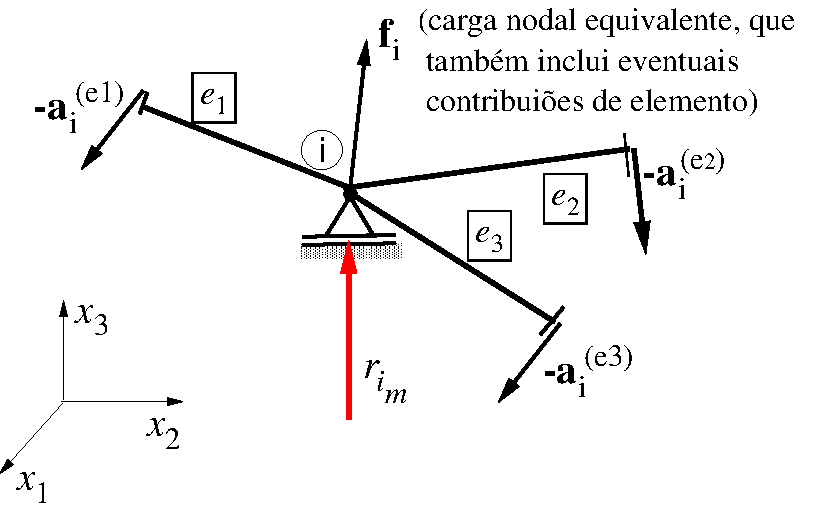
\includegraphics[scale=0.60]{img/reac1}
		\captionof{figure}{Reação de apoio segundo a direção \(i_m\) do nó \(i\).}   \vspace{12pt} \label{reac1}
	\end{minipage}
	\begin{minipage}{0.44\textwidth}  \vspace{-0.85cm}
		\[\mathbf{f}_i=\mathbf{f}_{ic} - \sum\limits_{j=1}^{nei}\mathbf{f}_{i0}^{(e_{ji})} \;\; \textrm{(caga nodal equivalente)} 	\]
	\end{minipage}%%% to prevent a space
\end{figure}
\noindent Por exemplo, para o caso indicado na Fig. \ref{reac1}, tem-se,  do equilíbrio na \(i_m\)-ésima direção:
\[f_{i_m}-\left( a_{i_m}^{(e_1)} + a_{i_m}^{(e_2)} + a_{i_m}^{(e_3)} \right)+r_{i_m}=r_{i_m}+f_{i_m}-\sum_{j=1}^{n}k_{i_mj}u_j=0 \, , \;\; \textrm{com}\;\; n\!=\!nno\cdot ndofn \, .\]
\noindent Assim, para essa direção, resultará (vide Eq. (\ref{reac0})):
\begin{equation} \label{recf}
	r_{i_m}=-f_{i_m}+\sum_{j=1}^{n}k_{i_mj}u_j=-f_{i_m}+f_{i_mr}^{(d)} \, .
\end{equation}

\noindent Note que, antes da introdução das condições de contorno segundo a técnica de "um e zeros", será necessário armazenar as linhas originais (não modificadas) \(k_{i_m j}\)  e \(f_{i_m}\), respectivamente, da matriz de rigidez e do vetor de cargas nodais equivalentes globais da estrutura. Para apoios elásticos, as reações de apoio podem ser diretamente calculadas via modelo matemático que descreve a mola. Tem-se, por exemplo:

\begin{equation} \label{rec_els}
	r_{i_m}=-k_{i_m}u_{i_m}
\end{equation}

\section{Esforços de Extremidade de Elemento}

Após introdução das condições de contorno e resolução do sistema de equações, de onde determinam-se os deslocamentos nodais da estrutura (referenciados ao sistema global), pode-se então calcular os esforços de extremidade de elemento. Para isso, usam-se as expressões (vide Fig. \ref{el_forces}), em que se considera um elemento de conectividades \(i\) e \(j\)):
\begin{equation} \label{esf_el1}
	{\mathbf{a'}}^{(e)}_{f}={\mathbf{f'}}^{(e)}_{0}+ {\mathbf{K'}}^{(e)}{\mathbf{u'}}^{(e)} \;\;,
\end{equation}
\noindent onde na eq. (\ref{esf_el1}), \({\mathbf{K'}}^{(e)}\) denota a matriz de rigidez do elemento \(e\) no referencial local, e os vetores \({\mathbf{f'}}^{(e)}_{0}\), \({\mathbf{u'}}^{(e)}\) e \({\mathbf{a'}}^{(e)}_f\), \(m\!=\!i,j\), contêm, respectivamente, as ações de engastamento perfeito de elemento no referencial local, os deslocamentos de elemento no referencial global e os valores finais dos esforços de extremidade de elemento. Em forma particionada (agrupando-se os graus de liberdade correspondentes a cada um dos nós), escreve-se, em termos das componentes globais de de deslocamentos:
\begin{equation} \label{esf_el2}
	\left\{ \begin{array}{rcl}
	{\mathbf{a'}}^{(e)}_{if} \!\!\!                      & = & \!\!\!
	                                        {\mathbf{f'}}^{(e)}_{i0}+ {\mathbf{K'}}^{(e)}_{ii} \left(\mathbf{R}^{(e)} \mathbf{u}^{(e)}_{i}\right) +{\mathbf{K'}}^{(e)}_{ij}\left(\mathbf{R}^{(e)} \mathbf{u}^{(e)}_{j}\right)                                                              \\
	                                        {\mathbf{a'}}^{(e)}_{jf} \!\!\! & = & \!\!\!  {\mathbf{f'}}^{(e)}_{j0} +
	                                                                                  {\mathbf{K'}}^{(e)}_{ji}\left(\mathbf{R}^{(e)} \mathbf{u}^{(e)}_{i}\right) + {\mathbf{K'}}^{(e)}_{jj}\left(\mathbf{R}^{(e)} \mathbf{u}^{(e)}_{j}\right)
	\end{array}  \right. \;\; ,
\end{equation}
\noindent onde os vetores \({\mathbf{f'}}^{(e)}_{m0}\), \(\mathbf{u}^{(e)}_{m}\) e \({\mathbf{a'}}^{(e)}_{mf}\), \(m\!=\!i,j\), contêm, respectivamente, associado ao nó \(m\), as ações de engastamento perfeito de elemento no referencial local, os deslocamentos de elemento no referencial global e os valores finais dos esforços de extremidade de elemento.
